\documentclass{beamer}

%------------------------------------------------
% Packages & Fonts
%------------------------------------------------
\usepackage[utf8]{inputenc}
\usepackage{graphicx}
\usepackage{xcolor}
\usepackage{tikz}
\usepackage{lmodern}
\usepackage{amsmath}
\usepackage{booktabs}
\usepackage{multirow}
\usepackage{appendixnumberbeamer}

%------------------------------------------------
% Stanford Colors
%------------------------------------------------
\definecolor{stanfordred}{HTML}{8C1515}
\definecolor{customlightgray}{rgb}{0.9,0.9,0.9}

%------------------------------------------------
% Theme & Color Overrides
%------------------------------------------------
\usetheme{Dresden}

\setbeamercolor{structure}{fg=stanfordred}
\setbeamercolor{title}{fg=stanfordred}
\setbeamercolor{frametitle}{bg=stanfordred, fg=white}
\setbeamercolor{itemize item}{fg=stanfordred}
\setbeamercolor{section in toc}{fg=stanfordred}
\setbeamertemplate{caption}[numbered]

% navigation dots in header/footer
\setbeamercolor{section in head/foot}{bg=customlightgray, fg=stanfordred}
\setbeamerfont{section in head/foot}{size=\scriptsize}

% turn off default nav symbols
\setbeamertemplate{navigation symbols}{}

%------------------------------------------------
% Custom Footline: only frame number
%------------------------------------------------
\setbeamertemplate{footline}{%
  \leavevmode%
  \hbox{%
    \hspace*{0.85\paperwidth}%
    \begin{beamercolorbox}[wd=0.15\paperwidth,ht=2.5ex,dp=1ex,right]{date in head/foot}%
      \insertframenumber{} / \inserttotalframenumber%
    \end{beamercolorbox}%
  }%
}

%------------------------------------------------
% Optional Stanford Logo on Every Slide
%------------------------------------------------
\IfFileExists{stanford_logo.png}{%
\addtobeamertemplate{frametitle}{}{%
\begin{tikzpicture}[remember picture,overlay]
    \node[anchor=north east,yshift=-25pt] at (current page.north east) {\includegraphics[height=0.6cm]{stanford_logo.png}};
\end{tikzpicture}%
}
}{%
% no logo file found
}
\setbeamerfont{frametitle}{size=\small}

%------------------------------------------------
% Document Info
%------------------------------------------------
\title{Local Nonlinear Projection-Based Reduced-Order Models}

\author{%
Sebastian Ares de Parga\textsuperscript{3}, \
Radek Tezaur\textsuperscript{1}, \
Charbel Farhat\textsuperscript{1,2} \
}

\institute{%
  \inst{1} Department of Aeronautics and Astronautics\\
  \inst{2} Institute for Computational and Mathematical Engineering\\
  Stanford University, Stanford, CA 94305, USA\\[0.5ex]
  \inst{3} CIMNE, Barcelona 08034, Spain\\[0.5ex]
}

\date{\today}

%------------------------------------------------
\begin{document}

\begin{frame}
  \titlepage
\end{frame}

\begin{frame}{Global ROM Storyline: LSPG + Gauss-Newton}
\small
Given the implicit HDM residual $\mathbf{r}(\mathbf{u})=\mathbf{0}$, define a manifold
\[
\mathbf{u}\approx \mathbf{u}_{\mathrm{ref}}+\widetilde{\mathbf{u}}(\mathbf{q}).
\]
LSPG solves at each time step:
\[
\mathbf{q}^{\star}
=\arg\min_{\mathbf{q}}\;
\frac{1}{2}\left\|\mathbf{r}\!\left(\mathbf{u}_{\mathrm{ref}}+\widetilde{\mathbf{u}}(\mathbf{q})\right)\right\|_2^2.
\]
With Gauss-Newton (current iterate $\mathbf{q}^{(k)}$), the increment $\Delta\mathbf{q}$ is obtained from
\[
\left(\mathbf{\Psi}^{T}\mathbf{J}^{T}\mathbf{J}\mathbf{\Psi}\right)\Delta\mathbf{q}
=-\mathbf{\Psi}^{T}\mathbf{J}^{T}\mathbf{r},
\]
where
\[
\mathbf{\Psi}=\frac{\partial\widetilde{\mathbf{u}}}{\partial\mathbf{q}},
\qquad
\mathbf{J}=\frac{\partial\mathbf{r}}{\partial\mathbf{u}},
\qquad
\mathbf{q}^{(k+1)}=\mathbf{q}^{(k)}+\Delta\mathbf{q}.
\]
\end{frame}

\begin{frame}{Global Linear PROM}
\small
State ansatz:
\[
\mathbf{u}\approx \mathbf{u}_{\mathrm{ref}}+\mathbf{V}\mathbf{q},
\qquad
\mathbf{V}\in\mathbb{R}^{N\times n},\; n=151.
\]
Hence
\[
\widetilde{\mathbf{u}}(\mathbf{q})=\mathbf{V}\mathbf{q},
\qquad
\mathbf{\Psi}=\frac{\partial\widetilde{\mathbf{u}}}{\partial\mathbf{q}}=\mathbf{V}.
\]
Gauss-Newton system:
\[
\left(\mathbf{V}^{T}\mathbf{J}^{T}\mathbf{J}\mathbf{V}\right)\Delta\mathbf{q}
=-\mathbf{V}^{T}\mathbf{J}^{T}\mathbf{r}.
\]
\end{frame}

\begin{frame}{Global QPROM}
\small
Quadratic-manifold ansatz:
\[
\mathbf{u}\approx
\mathbf{u}_{\mathrm{ref}}
+\mathbf{V}\mathbf{q}
+\mathbf{H}\left(\mathbf{q}\otimes\mathbf{q}\right),
\qquad
n=16.
\]
Thus
\[
\widetilde{\mathbf{u}}(\mathbf{q})
=\mathbf{V}\mathbf{q}
+\mathbf{H}\left(\mathbf{q}\otimes\mathbf{q}\right),
\]
and the tangent depends on the current reduced state:
\[
\mathbf{\Psi}(\mathbf{q})
=\frac{\partial\widetilde{\mathbf{u}}}{\partial\mathbf{q}}
=\mathbf{V}
+\frac{\partial}{\partial\mathbf{q}}
\!\left[\mathbf{H}\left(\mathbf{q}\otimes\mathbf{q}\right)\right].
\]
\end{frame}

\begin{frame}{Global PROM-GPR}
\small
Split basis and reduced coordinates:
\[
\mathbf{V}_{\mathrm{tot}}=[\mathbf{V},\bar{\mathbf{V}}],
\qquad
\mathbf{q}_{\mathrm{tot}}=
\begin{bmatrix}
\mathbf{q}\\
\bar{\mathbf{q}}
\end{bmatrix}.
\]
\[
\bar{\mathbf{q}}=\mathcal{N}_{\mathrm{GPR}}(\mathbf{q}),
\qquad
n=10,\;\bar{n}=141.
\]
State ansatz:
\[
\mathbf{u}\approx
\mathbf{u}_{\mathrm{ref}}
+\widetilde{\mathbf{u}}(\mathbf{q}),
\]
\[
\widetilde{\mathbf{u}}(\mathbf{q})
=\mathbf{V}_{\mathrm{tot}}\mathbf{q}_{\mathrm{tot}}
=\mathbf{V}\mathbf{q}
+\bar{\mathbf{V}}\,\mathcal{N}_{\mathrm{GPR}}(\mathbf{q}).
\]
Effective tangent for Gauss-Newton:
\[
\mathbf{\Psi}(\mathbf{q})
=\frac{\partial\widetilde{\mathbf{u}}}{\partial\mathbf{q}}
=\mathbf{V}
+\bar{\mathbf{V}}\frac{\partial\mathcal{N}_{\mathrm{GPR}}}{\partial\mathbf{q}}.
\]
\end{frame}

\begin{frame}{Global PROM-POD-DL}
\small
Latent reduced coordinate $\mathbf{z}\in\mathbb{R}^{5}$ with learned map:
\[
\mathbf{q}_{\mathrm{tot}}=\mathcal{N}_{\mathrm{DL}}(\mathbf{z}),
\qquad
\mathbf{q}_{\mathrm{tot}}\in\mathbb{R}^{151}.
\]
State reconstruction:
\[
\mathbf{u}\approx
\mathbf{u}_{\mathrm{ref}}
+\widetilde{\mathbf{u}}(\mathbf{z}),
\]
\[
\widetilde{\mathbf{u}}(\mathbf{z})
=\mathbf{V}_{\mathrm{tot}}\mathbf{q}_{\mathrm{tot}}
=\mathbf{V}_{\mathrm{tot}}\mathcal{N}_{\mathrm{DL}}(\mathbf{z}),
\qquad
\mathbf{V}_{\mathrm{tot}}\in\mathbb{R}^{N\times 151}.
\]
Effective tangent for Gauss-Newton:
\[
\mathbf{\Psi}(\mathbf{z})
=\frac{\partial\widetilde{\mathbf{u}}}{\partial\mathbf{z}}
=\mathbf{V}_{\mathrm{tot}}
\frac{\partial\mathcal{N}_{\mathrm{DL}}}{\partial\mathbf{z}}.
\]
\end{frame}

\begin{frame}{Local ROMs: piecewise manifolds}
\small

Partition the training snapshots into clusters $k=1,\dots,N_c$ and build one local trial manifold per cluster:
\[
\mathbf u \approx \Phi_k(\mathbf q_k).
\]

Examples used in this work:
\[
\Phi_k^{\mathrm{lin}}(\mathbf q)
=
\mathbf u_{0,k}+\mathbf V_k\mathbf q,
\]
\[
\Phi_k^{\mathrm{quad}}(\mathbf q)
=
\mathbf u_{0,k}+\mathbf V_k\mathbf q+\mathbf H_k(\mathbf q\otimes\mathbf q),
\]
\[
\Phi_k^{\mathrm{gpr}}(\mathbf q)
=
\mathbf u_{0,k}+\mathbf V_k\mathbf q+\bar{\mathbf V}_k\,\mathcal N_{\mathrm{GPR},k}(\mathbf q).
\]

\vspace{0.3em}
\textbf{Online workflow}
\begin{enumerate}
    \item Select the active cluster.
    \item If the cluster changes, transfer the current state to the new local manifold.
    \item Solve the local LSPG problem in the active manifold.
\end{enumerate}

\vspace{0.3em}
In the next slides, we focus only on steps 1 and 2.

\end{frame}

\begin{frame}{Cheap Cluster Selection (1/2)}
\scriptsize
Current active cluster $k^-$, current local coordinates $\mathbf q_{k^-}$:
\[
\mathbf u^s=\mathbf u_{0,k^-}+\mathbf V_{k^-}\mathbf q_{k^-}.
\]
Choose the next cluster by nearest centroid:
\[
k^+=\arg\min_{\ell\in\{1,\dots,N_c\}}
\|\mathbf u^s-\mathbf u_{c,\ell}\|_2^2.
\]
Distance expansion:
\[
\|\mathbf u^s-\mathbf u_{c,\ell}\|_2^2
=
\|\mathbf q_{k^-}\|_2^2
+2(\mathbf u_{0,k^-}-\mathbf u_{c,\ell})^T\mathbf V_{k^-}\mathbf q_{k^-}
+\|\mathbf u_{0,k^-}-\mathbf u_{c,\ell}\|_2^2.
\]
Offline precompute:
\[
\mathbf g_{k^-,\ell}:=\mathbf V_{k^-}^T(\mathbf u_{0,k^-}-\mathbf u_{c,\ell}),
\qquad
d_{k^-,\ell}:=\|\mathbf u_{0,k^-}-\mathbf u_{c,\ell}\|_2^2.
\]
\end{frame}

\begin{frame}{Cheap Cluster Selection (2/2)}
\scriptsize
Online selector:
\[
k^+=\arg\min_{\ell}
\left(2\,\mathbf g_{k^-,\ell}^T\mathbf q_{k^-}+d_{k^-,\ell}\right),
\]
since $\|\mathbf q_{k^-}\|_2^2$ is independent of $\ell$.

\vspace{0.4em}
\textbf{Switch decision}
\[
k^+=k^- \;\Rightarrow\; \text{no transfer},
\qquad
k^+\neq k^- \;\Rightarrow\; \text{solve switch projection}.
\]

\vspace{0.4em}
\textbf{Current strategy}
\begin{itemize}
\item Local PROM: selector used directly.
\item Local QPROM and local PROM-GPR: same cheap selector reused to keep switching inexpensive and robust.
\end{itemize}
\end{frame}

\begin{frame}{State Transfer After Cluster Switch (Linear)}
\scriptsize
Transferred state:
\[
\mathbf u^s=\mathbf u_{0,k^-}+\mathbf V_{k^-}\mathbf q_{k^-}.
\]
If new cluster $k^+$ uses an affine manifold,
\[
\mathbf u\approx \mathbf u_{0,k^+}+\mathbf V_{k^+}\mathbf q,
\]
compute new coordinates by least squares:
\[
\mathbf q_{k^+}
=
\arg\min_{\mathbf q}
\left\|
\mathbf u^s-(\mathbf u_{0,k^+}+\mathbf V_{k^+}\mathbf q)
\right\|_2^2.
\]
If $\mathbf V_{k^+}^T\mathbf V_{k^+}=\mathbf I$:
\[
\mathbf q_{k^+}
=\mathbf V_{k^+}^T
\left(
\mathbf u_{0,k^-}+\mathbf V_{k^-}\mathbf q_{k^-}-\mathbf u_{0,k^+}
\right).
\]
\end{frame}

\begin{frame}{State Transfer After Cluster Switch (Nonlinear)}
\scriptsize
If new cluster $k^+$ uses a nonlinear manifold
\[
\mathbf u\approx \Phi_{k^+}(\mathbf q),
\]
the switch projection is nonlinear least squares:
\[
\mathbf q_{k^+}
=\arg\min_{\mathbf q}
\left\|
\mathbf u^s-\Phi_{k^+}(\mathbf q)
\right\|_2^2.
\]
With
\[
\mathbf J_{\Phi}(\mathbf q):=\frac{\partial\Phi_{k^+}}{\partial\mathbf q},
\]
a Gauss--Newton step at iterate $\mathbf q^{(j)}$ is
\[
\left(\mathbf J_{\Phi}^T\mathbf J_{\Phi}\right)\Delta\mathbf q
=
\mathbf J_{\Phi}^T\left(\mathbf u^s-\Phi_{k^+}(\mathbf q^{(j)})\right),
\qquad
\mathbf q^{(j+1)}=\mathbf q^{(j)}+\Delta\mathbf q.
\]

\vspace{0.4em}
\textbf{At each switch}:
\begin{itemize}
\item linear local model $\Rightarrow$ linear least-squares transfer,
\item nonlinear local model $\Rightarrow$ nonlinear least-squares transfer.
\end{itemize}
\end{frame}

\begin{frame}{Online Performance ($250\times250$): $\boldsymbol{\mu}=(4.56,\,0.019)$}
\scriptsize
\centering
\resizebox{\textwidth}{!}{%
\begin{tabular}{lrrrrr}
\hline
\textbf{Computational model} & $n$ ($N$ for HDM) & $\bar{n}$ (or $n_{\mathrm{tot}}$ for POD-DL) & $\mathbb{RE}_{2,\mathbf{u}}$ (\%) & Wall-clock time (min) & Speedup \\
\hline
HDM & 125\,000 & -- & -- & 12.512 & -- \\
\addlinespace[0.35em]
PROM & 151 & -- & 0.450 & 5.934 & 2.108 \\
QPROM & 16 & -- & 6.563 & 3.725 & 3.359 \\
PROM-GPR & 10 & 141 & 2.112 & 2.374 & 5.269 \\
PROM-POD-DL & 5 & $n_{\mathrm{tot}}=151$ & 1.242 & 2.116 & 5.914 \\
\addlinespace[0.35em]
Local PROM ($N_c=10$) & 24--47 & -- & 0.195 & 3.929 & 3.184 \\
Local QPROM ($N_c=10$) & 6--9 & -- & 2.605 & 1.806 & 6.928 \\
Local PROM-GPR ($N_c=10$) & 5 & 24--47 & 0.823 & 1.701 & 7.357 \\
\hline
\end{tabular}}
\vspace{0.2em}

{\tiny Speedup is computed with respect to the HDM runtime, $t_{\mathrm{HDM}}=750.702$ s.}

{\tiny For PROM-POD-DL, $n=5$ is the latent dimension and $n_{\mathrm{tot}}=151$ is the decoded coordinate size.}

{\tiny All local models use $N_c=10$ clusters.}
\end{frame}

\begin{frame}{PROM Solution ($250\times250$): $\boldsymbol{\mu}=(4.56,\,0.019)$}
\centering
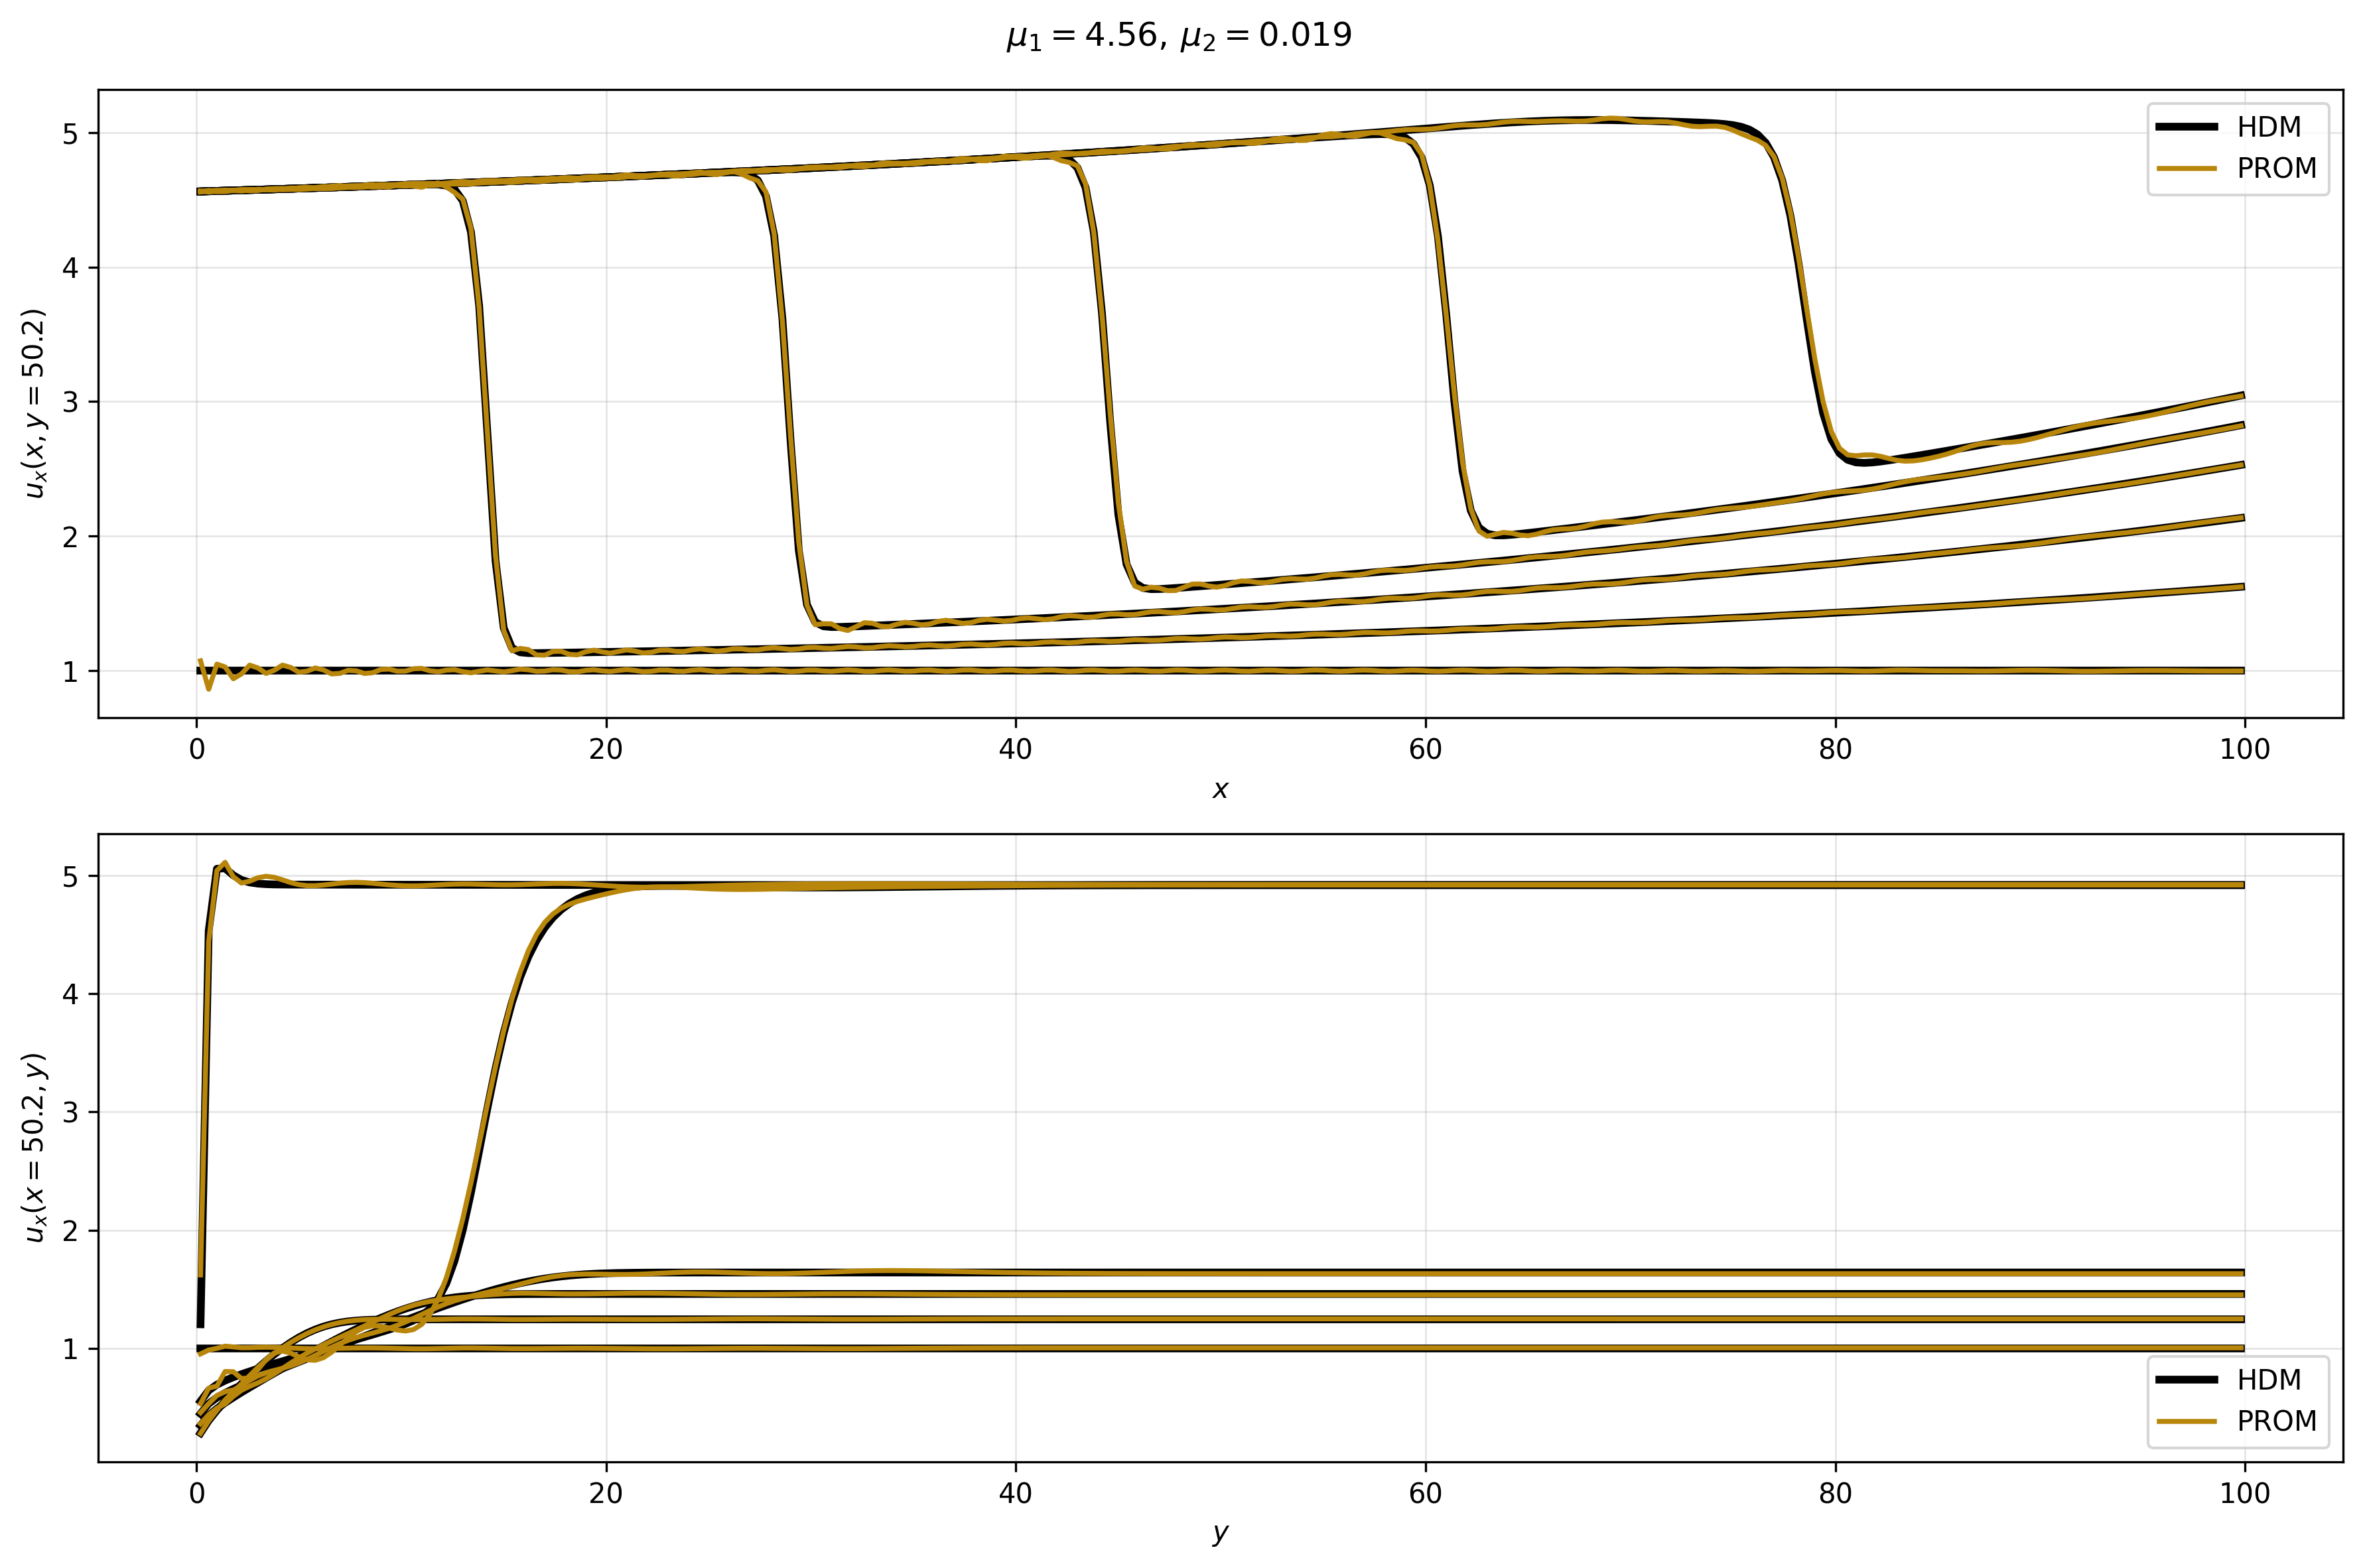
\includegraphics[width=0.80\textwidth]{Figures/prom_vs_hdm.png}
\vspace{0.2em}

{\scriptsize $\mathbb{RE}_{2,\mathbf{u}}=0.450\%$ \quad $t=356.059$ s $(5.934$ min$)$ \quad speedup $=2.108\times$}
\end{frame}

\begin{frame}{Local PROM Solution ($250\times250$): $\boldsymbol{\mu}=(4.56,\,0.019)$}
\centering
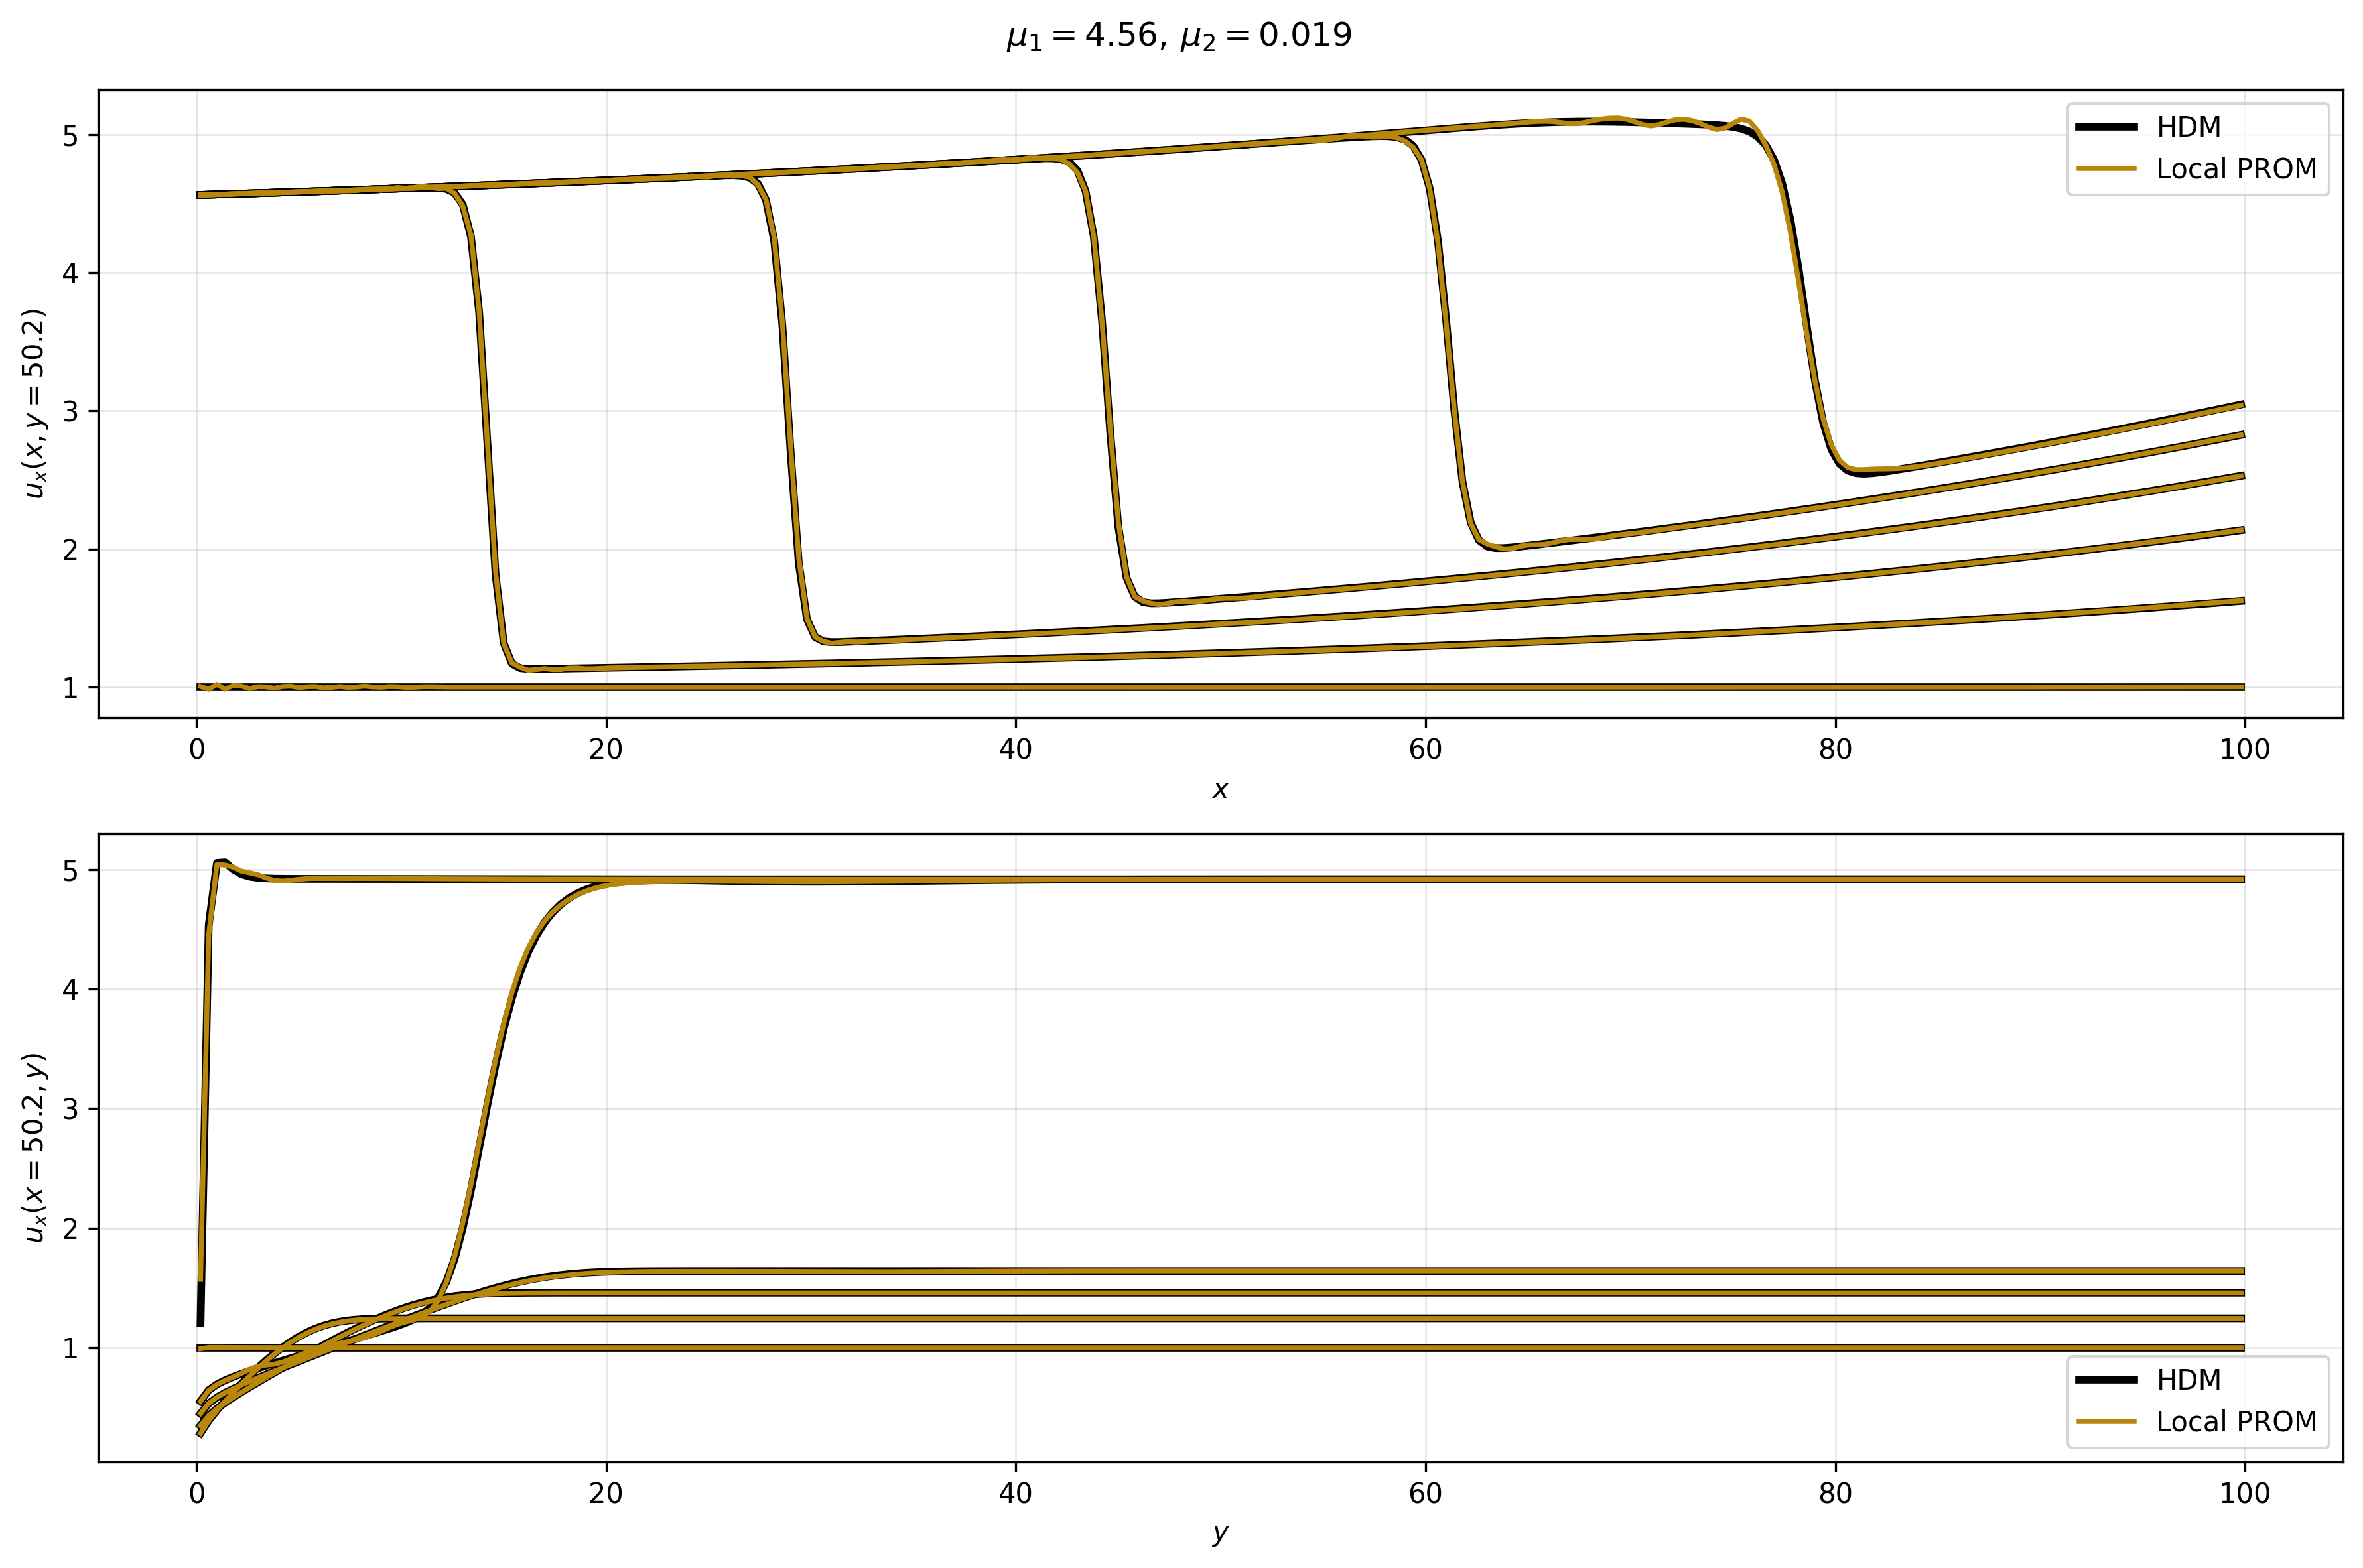
\includegraphics[width=0.80\textwidth]{Figures/local_prom_vs_hdm.png}
\vspace{0.2em}

{\scriptsize $\mathbb{RE}_{2,\mathbf{u}}=0.195\%$ \quad $t=235.750$ s $(3.929$ min$)$ \quad speedup $=3.184\times$}
\end{frame}

\begin{frame}{QPROM Solution ($250\times250$): $\boldsymbol{\mu}=(4.56,\,0.019)$}
\centering
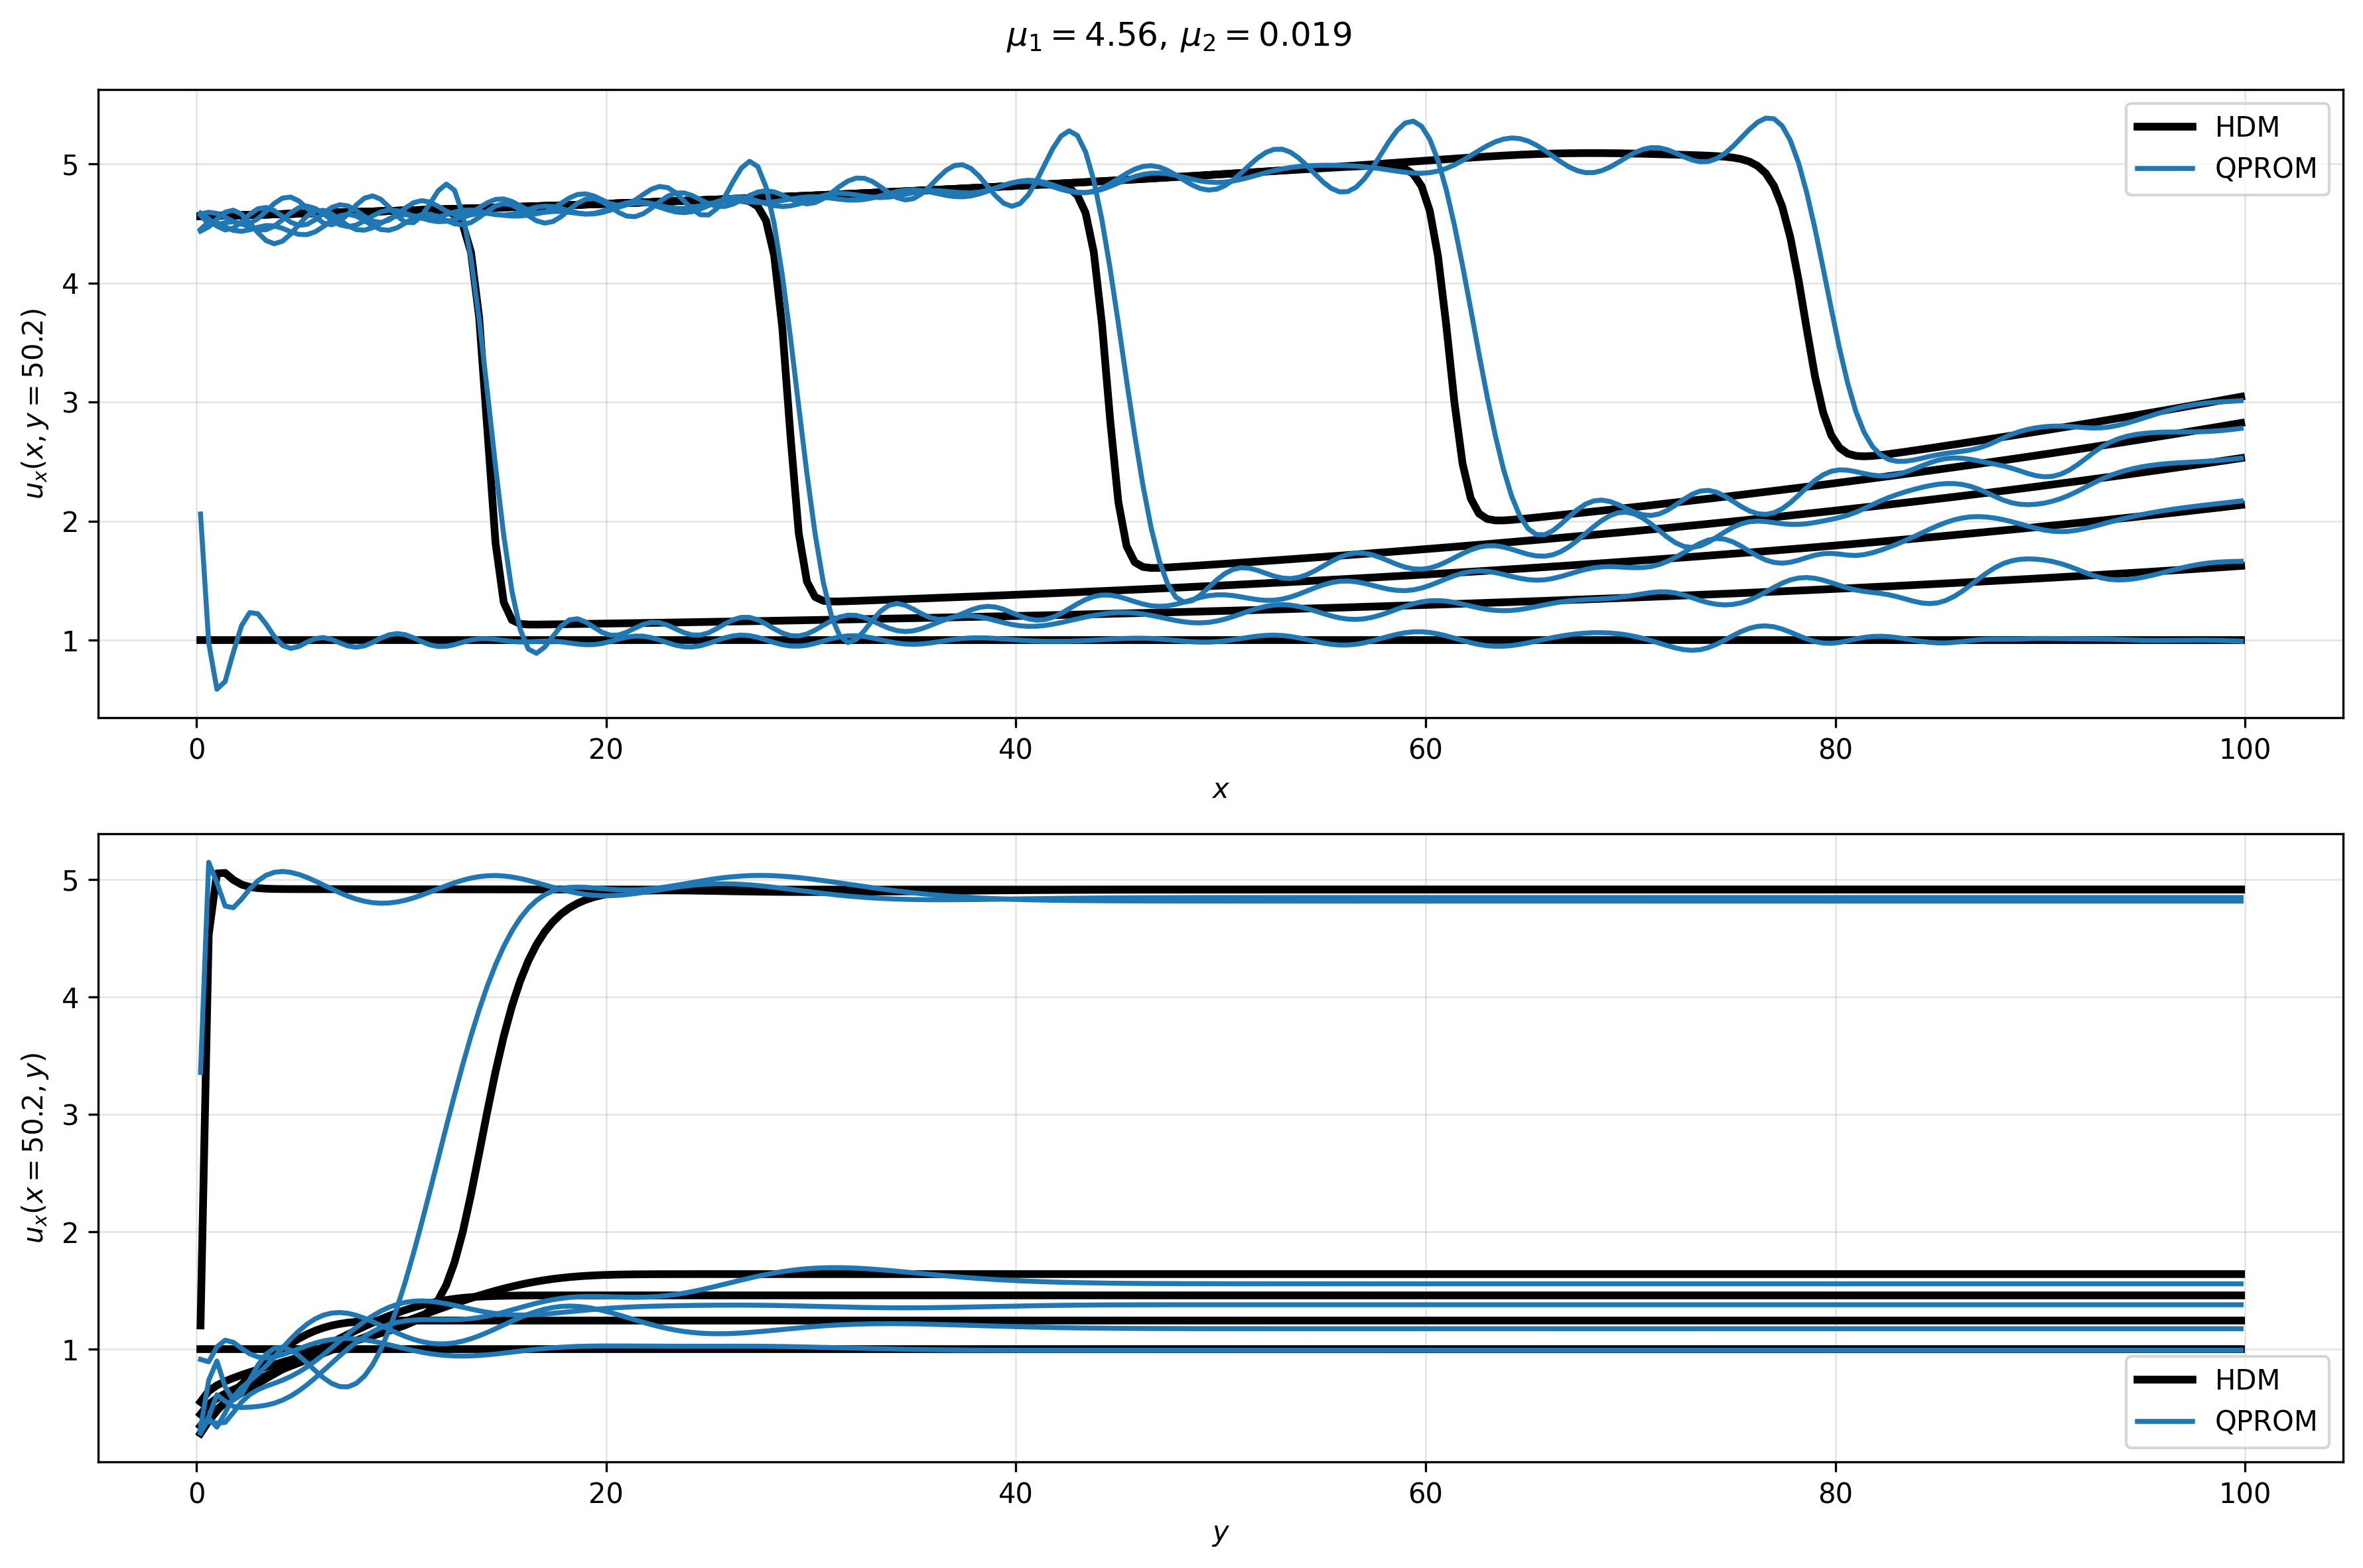
\includegraphics[width=0.80\textwidth]{Figures/qprom_vs_hdm.png}
\vspace{0.2em}

{\scriptsize $\mathbb{RE}_{2,\mathbf{u}}=6.563\%$ \quad $t=223.516$ s $(3.725$ min$)$ \quad speedup $=3.359\times$}
\end{frame}

\begin{frame}{Local QPROM Solution ($250\times250$): $\boldsymbol{\mu}=(4.56,\,0.019)$}
\centering
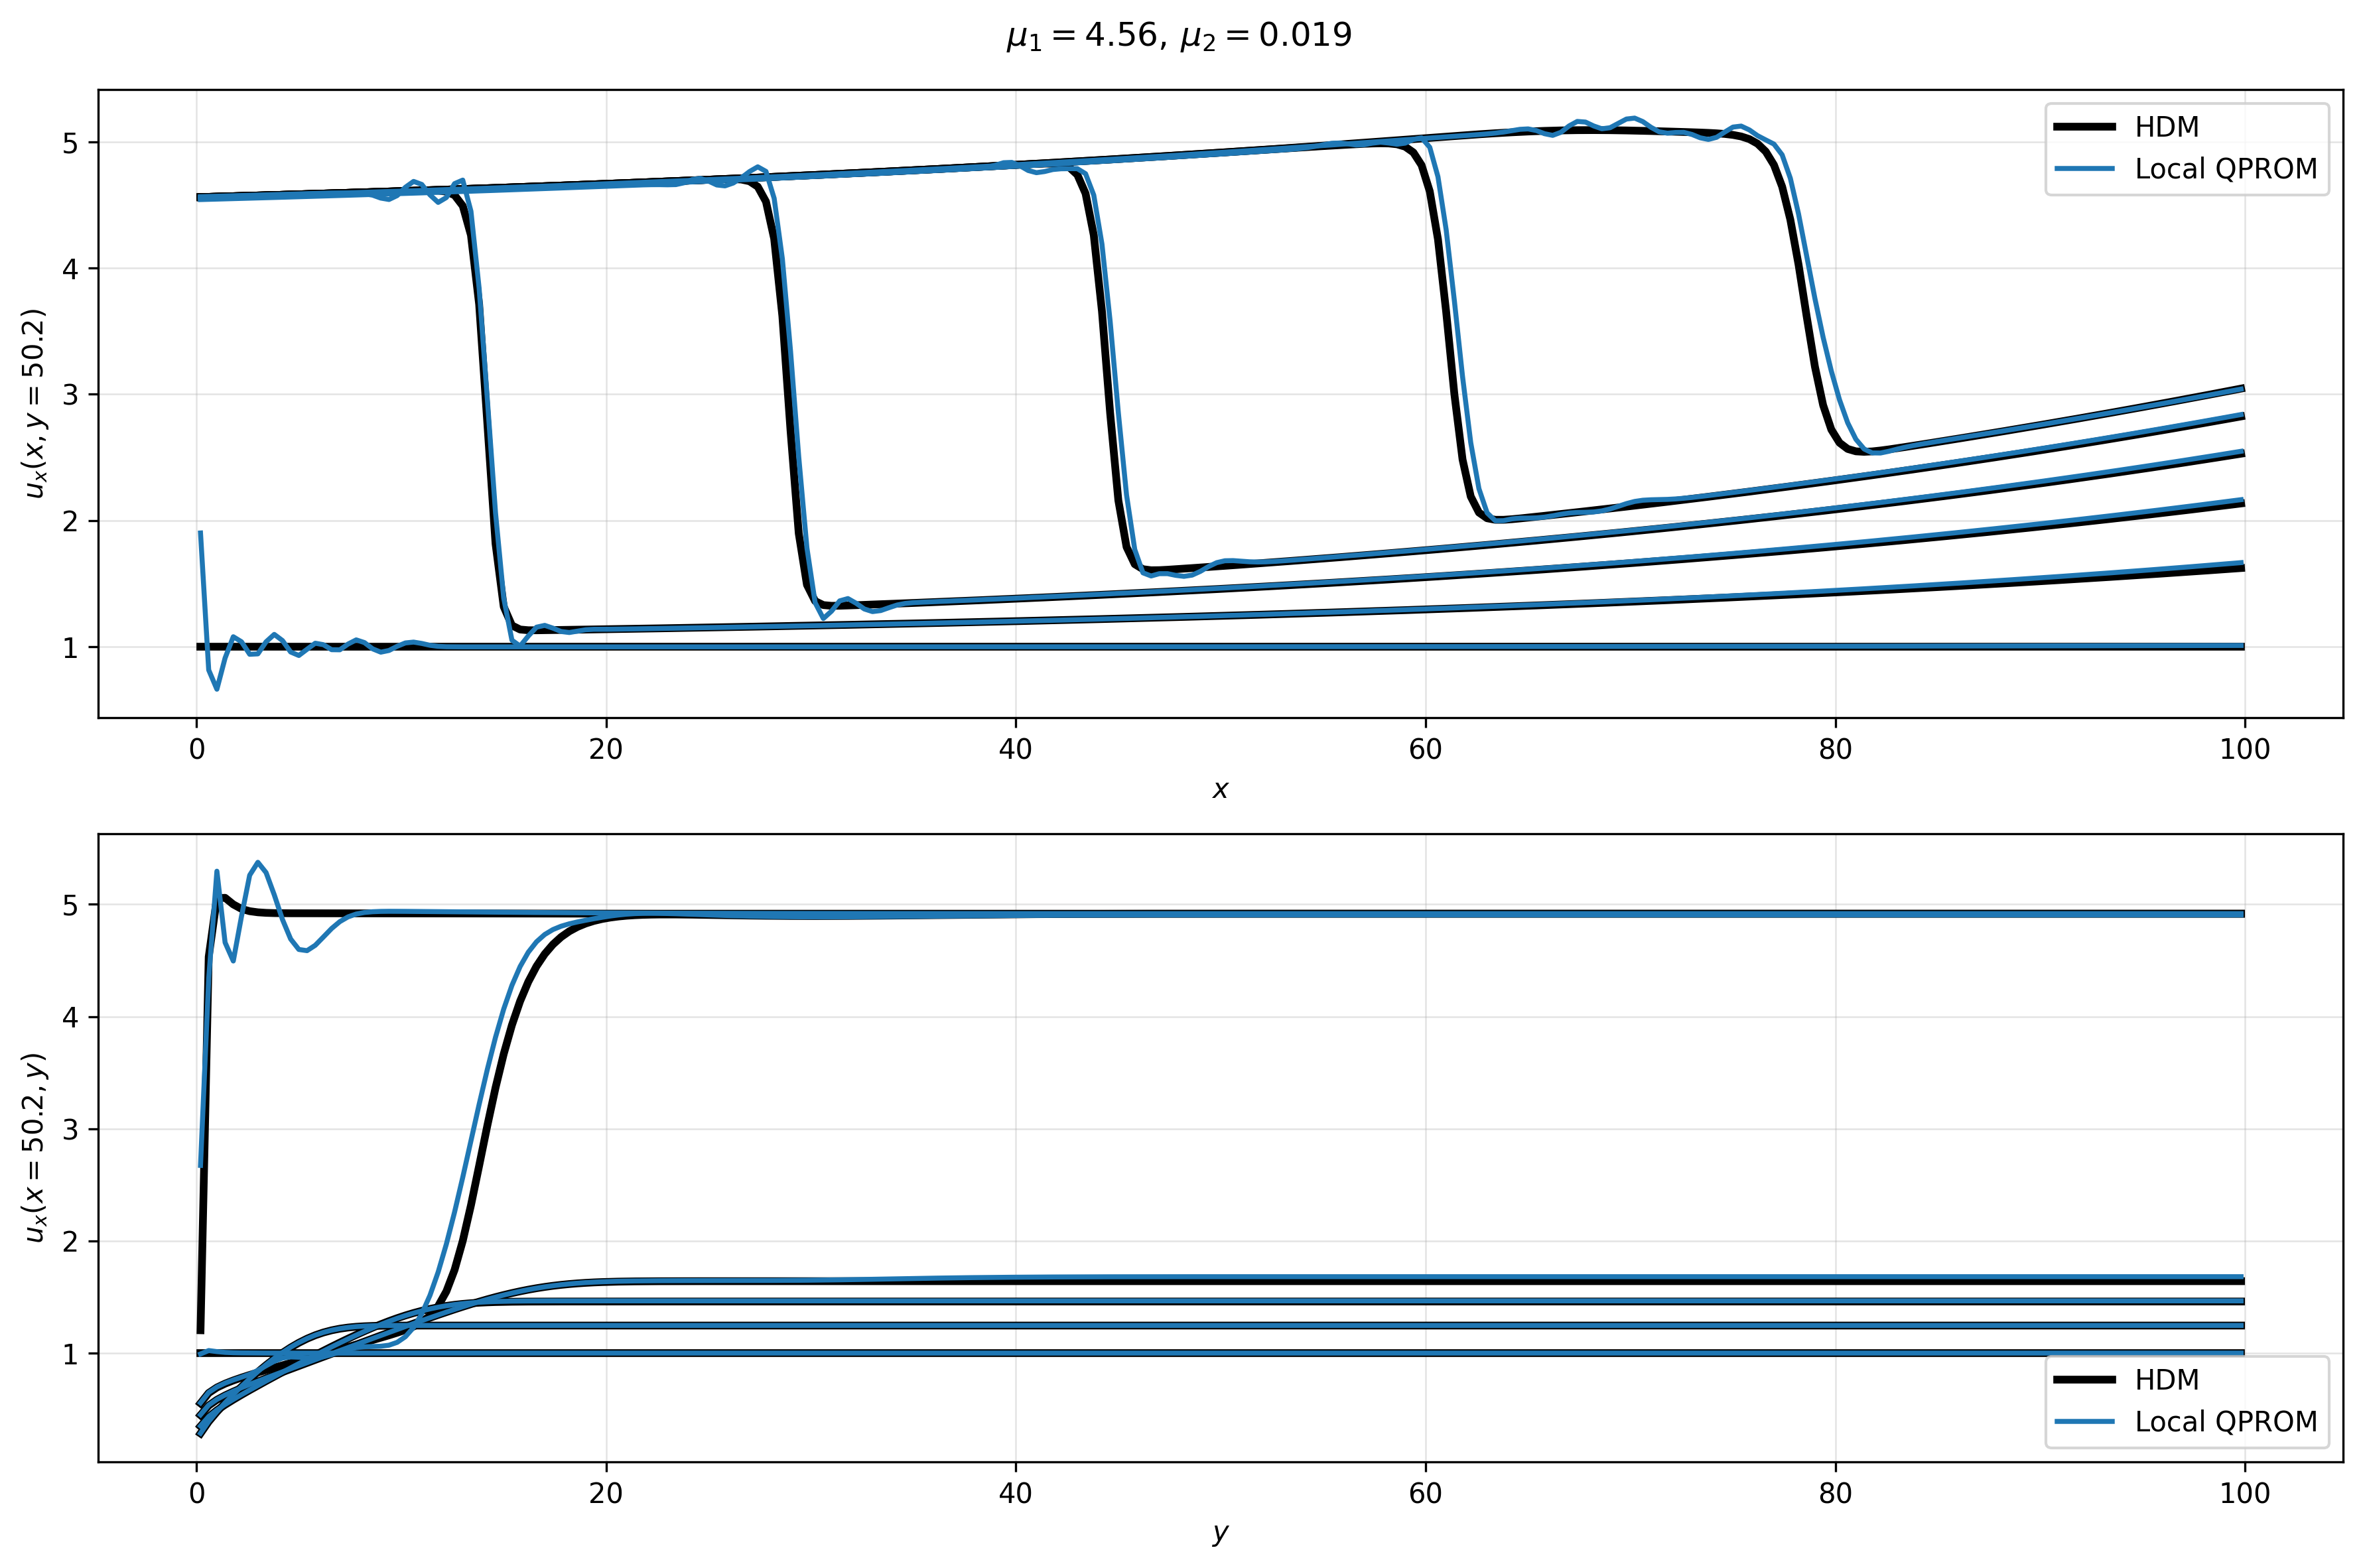
\includegraphics[width=0.80\textwidth]{Figures/local_qprom_vs_hdm.png}
\vspace{0.2em}

{\scriptsize $\mathbb{RE}_{2,\mathbf{u}}=2.605\%$ \quad $t=108.365$ s $(1.806$ min$)$ \quad speedup $=6.928\times$}
\end{frame}

\begin{frame}{PROM-GPR Solution ($250\times250$): $\boldsymbol{\mu}=(4.56,\,0.019)$}
\centering
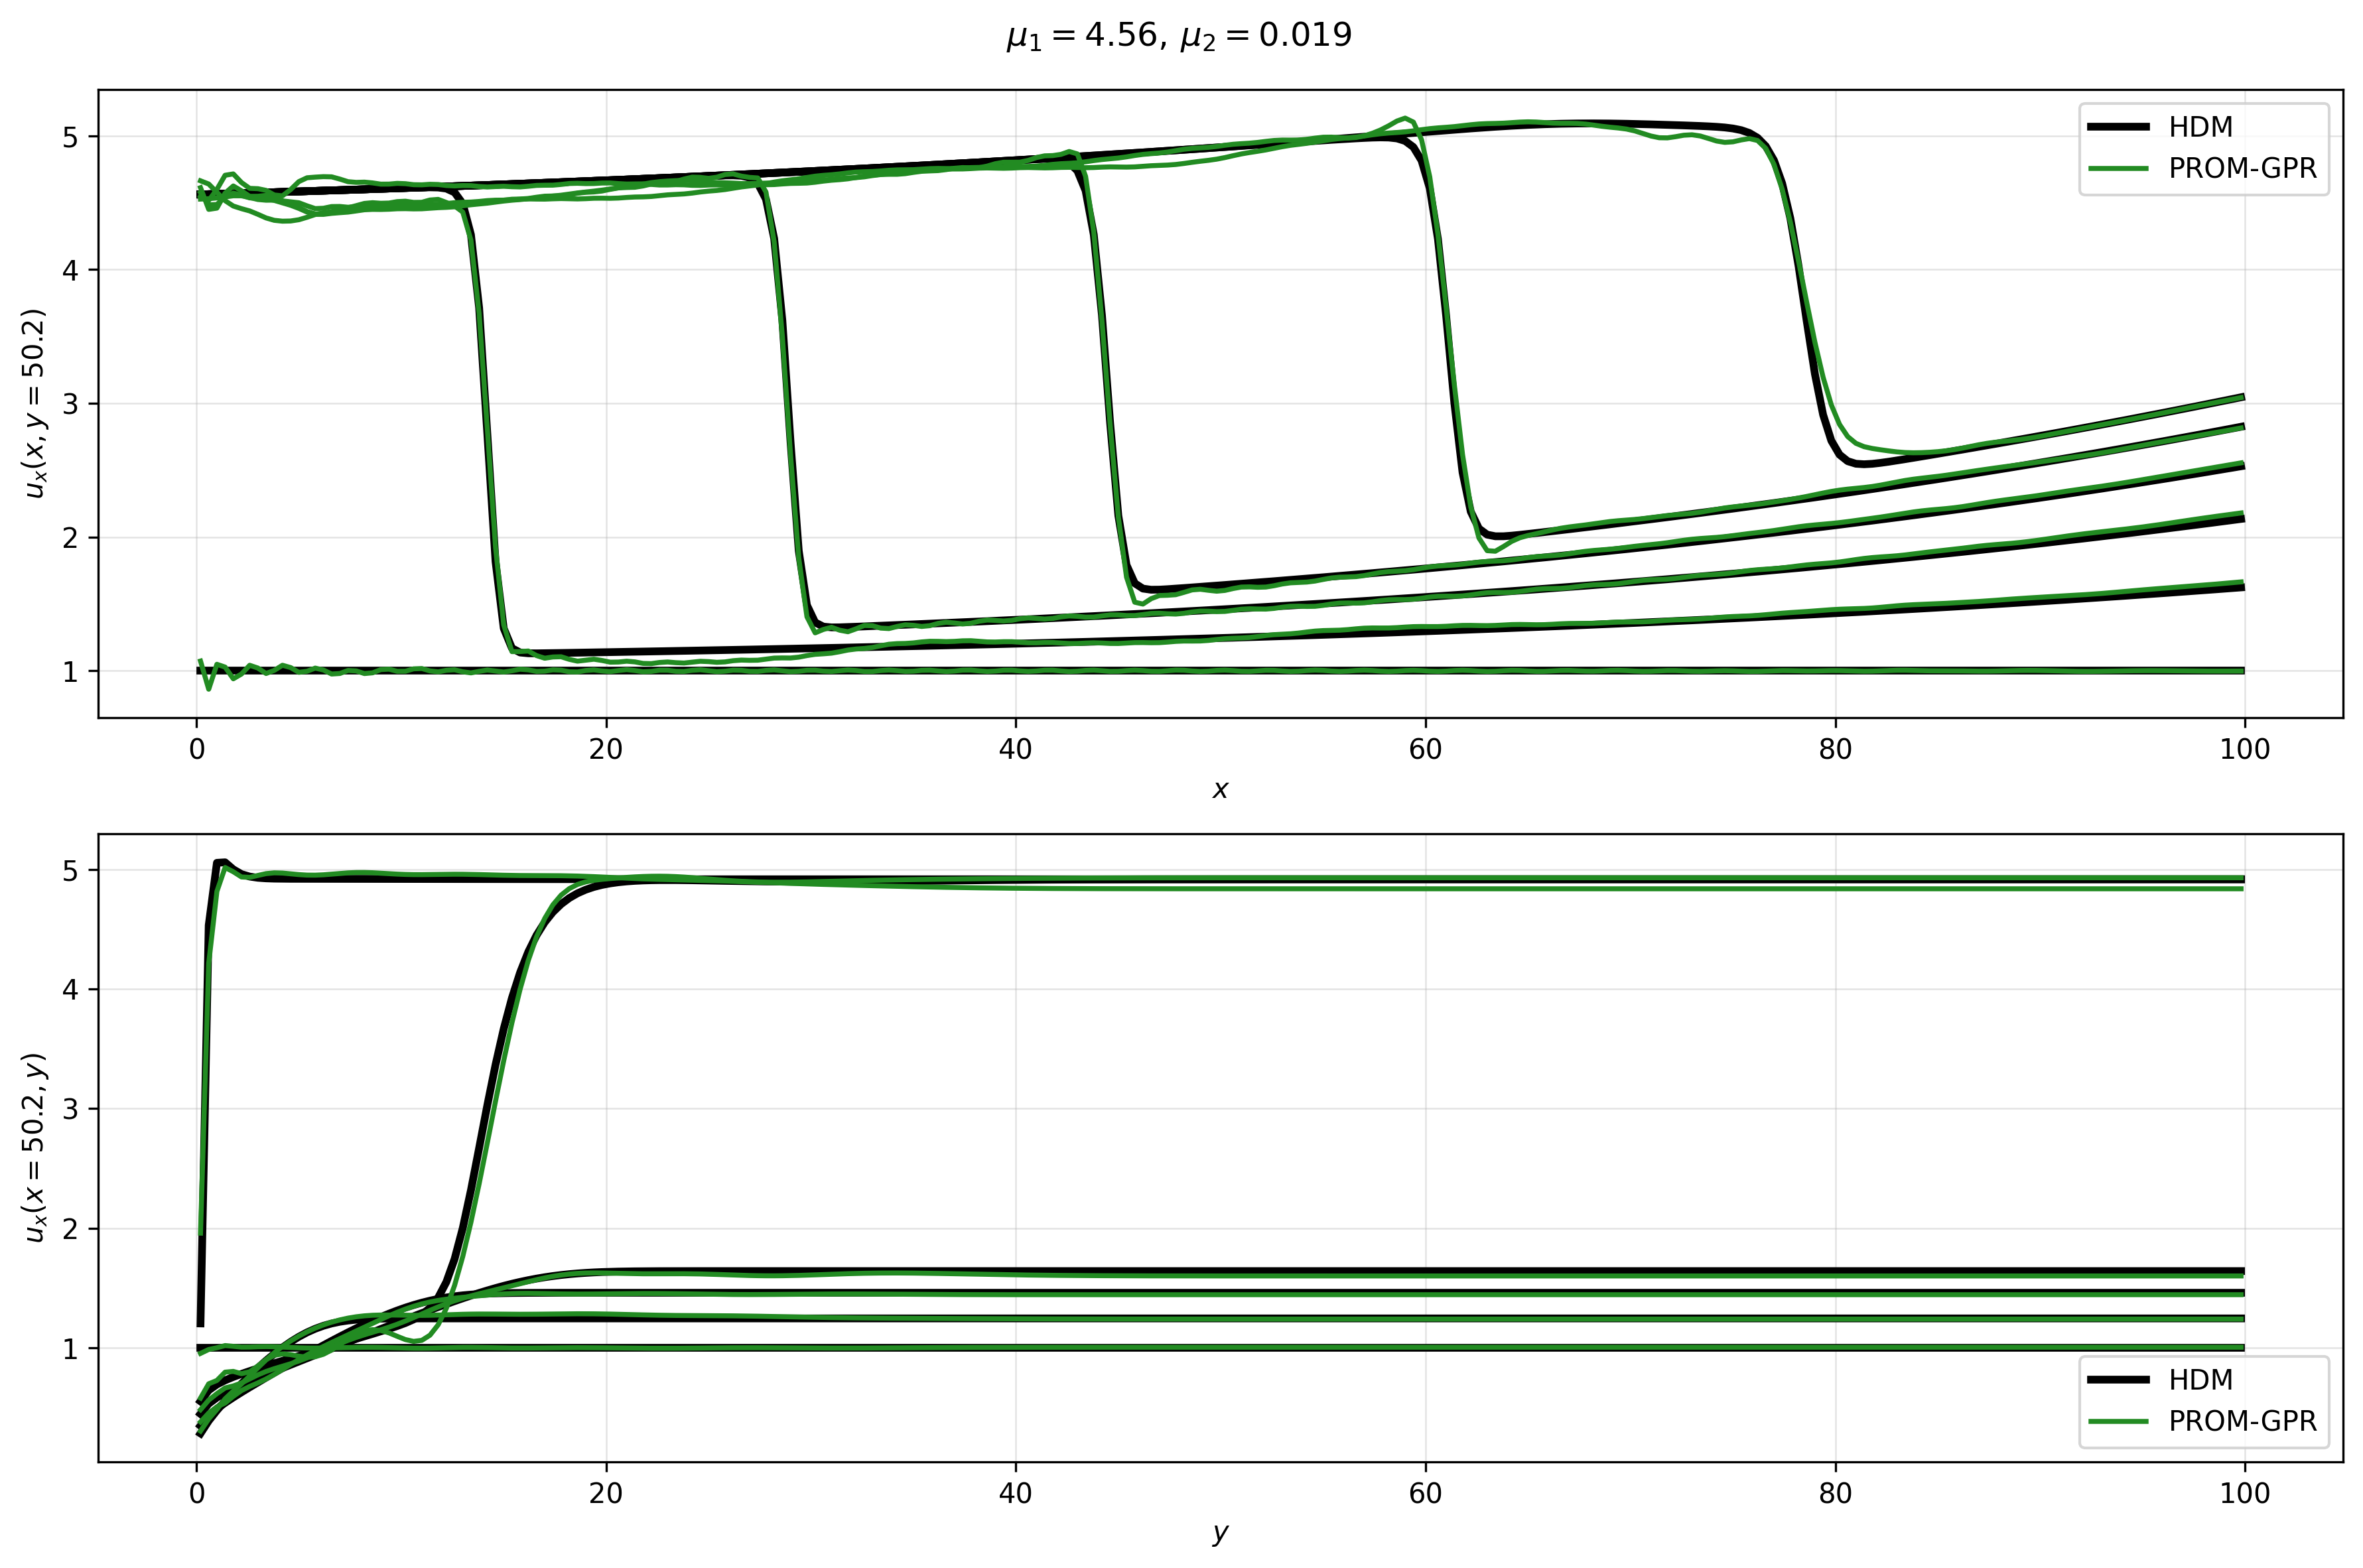
\includegraphics[width=0.80\textwidth]{Figures/prom_gpr_vs_hdm.png}
\vspace{0.2em}

{\scriptsize $\mathbb{RE}_{2,\mathbf{u}}=2.112\%$ \quad $t=142.463$ s $(2.374$ min$)$ \quad speedup $=5.269\times$}
\end{frame}

\begin{frame}{Local PROM-GPR Solution ($250\times250$): $\boldsymbol{\mu}=(4.56,\,0.019)$}
\centering
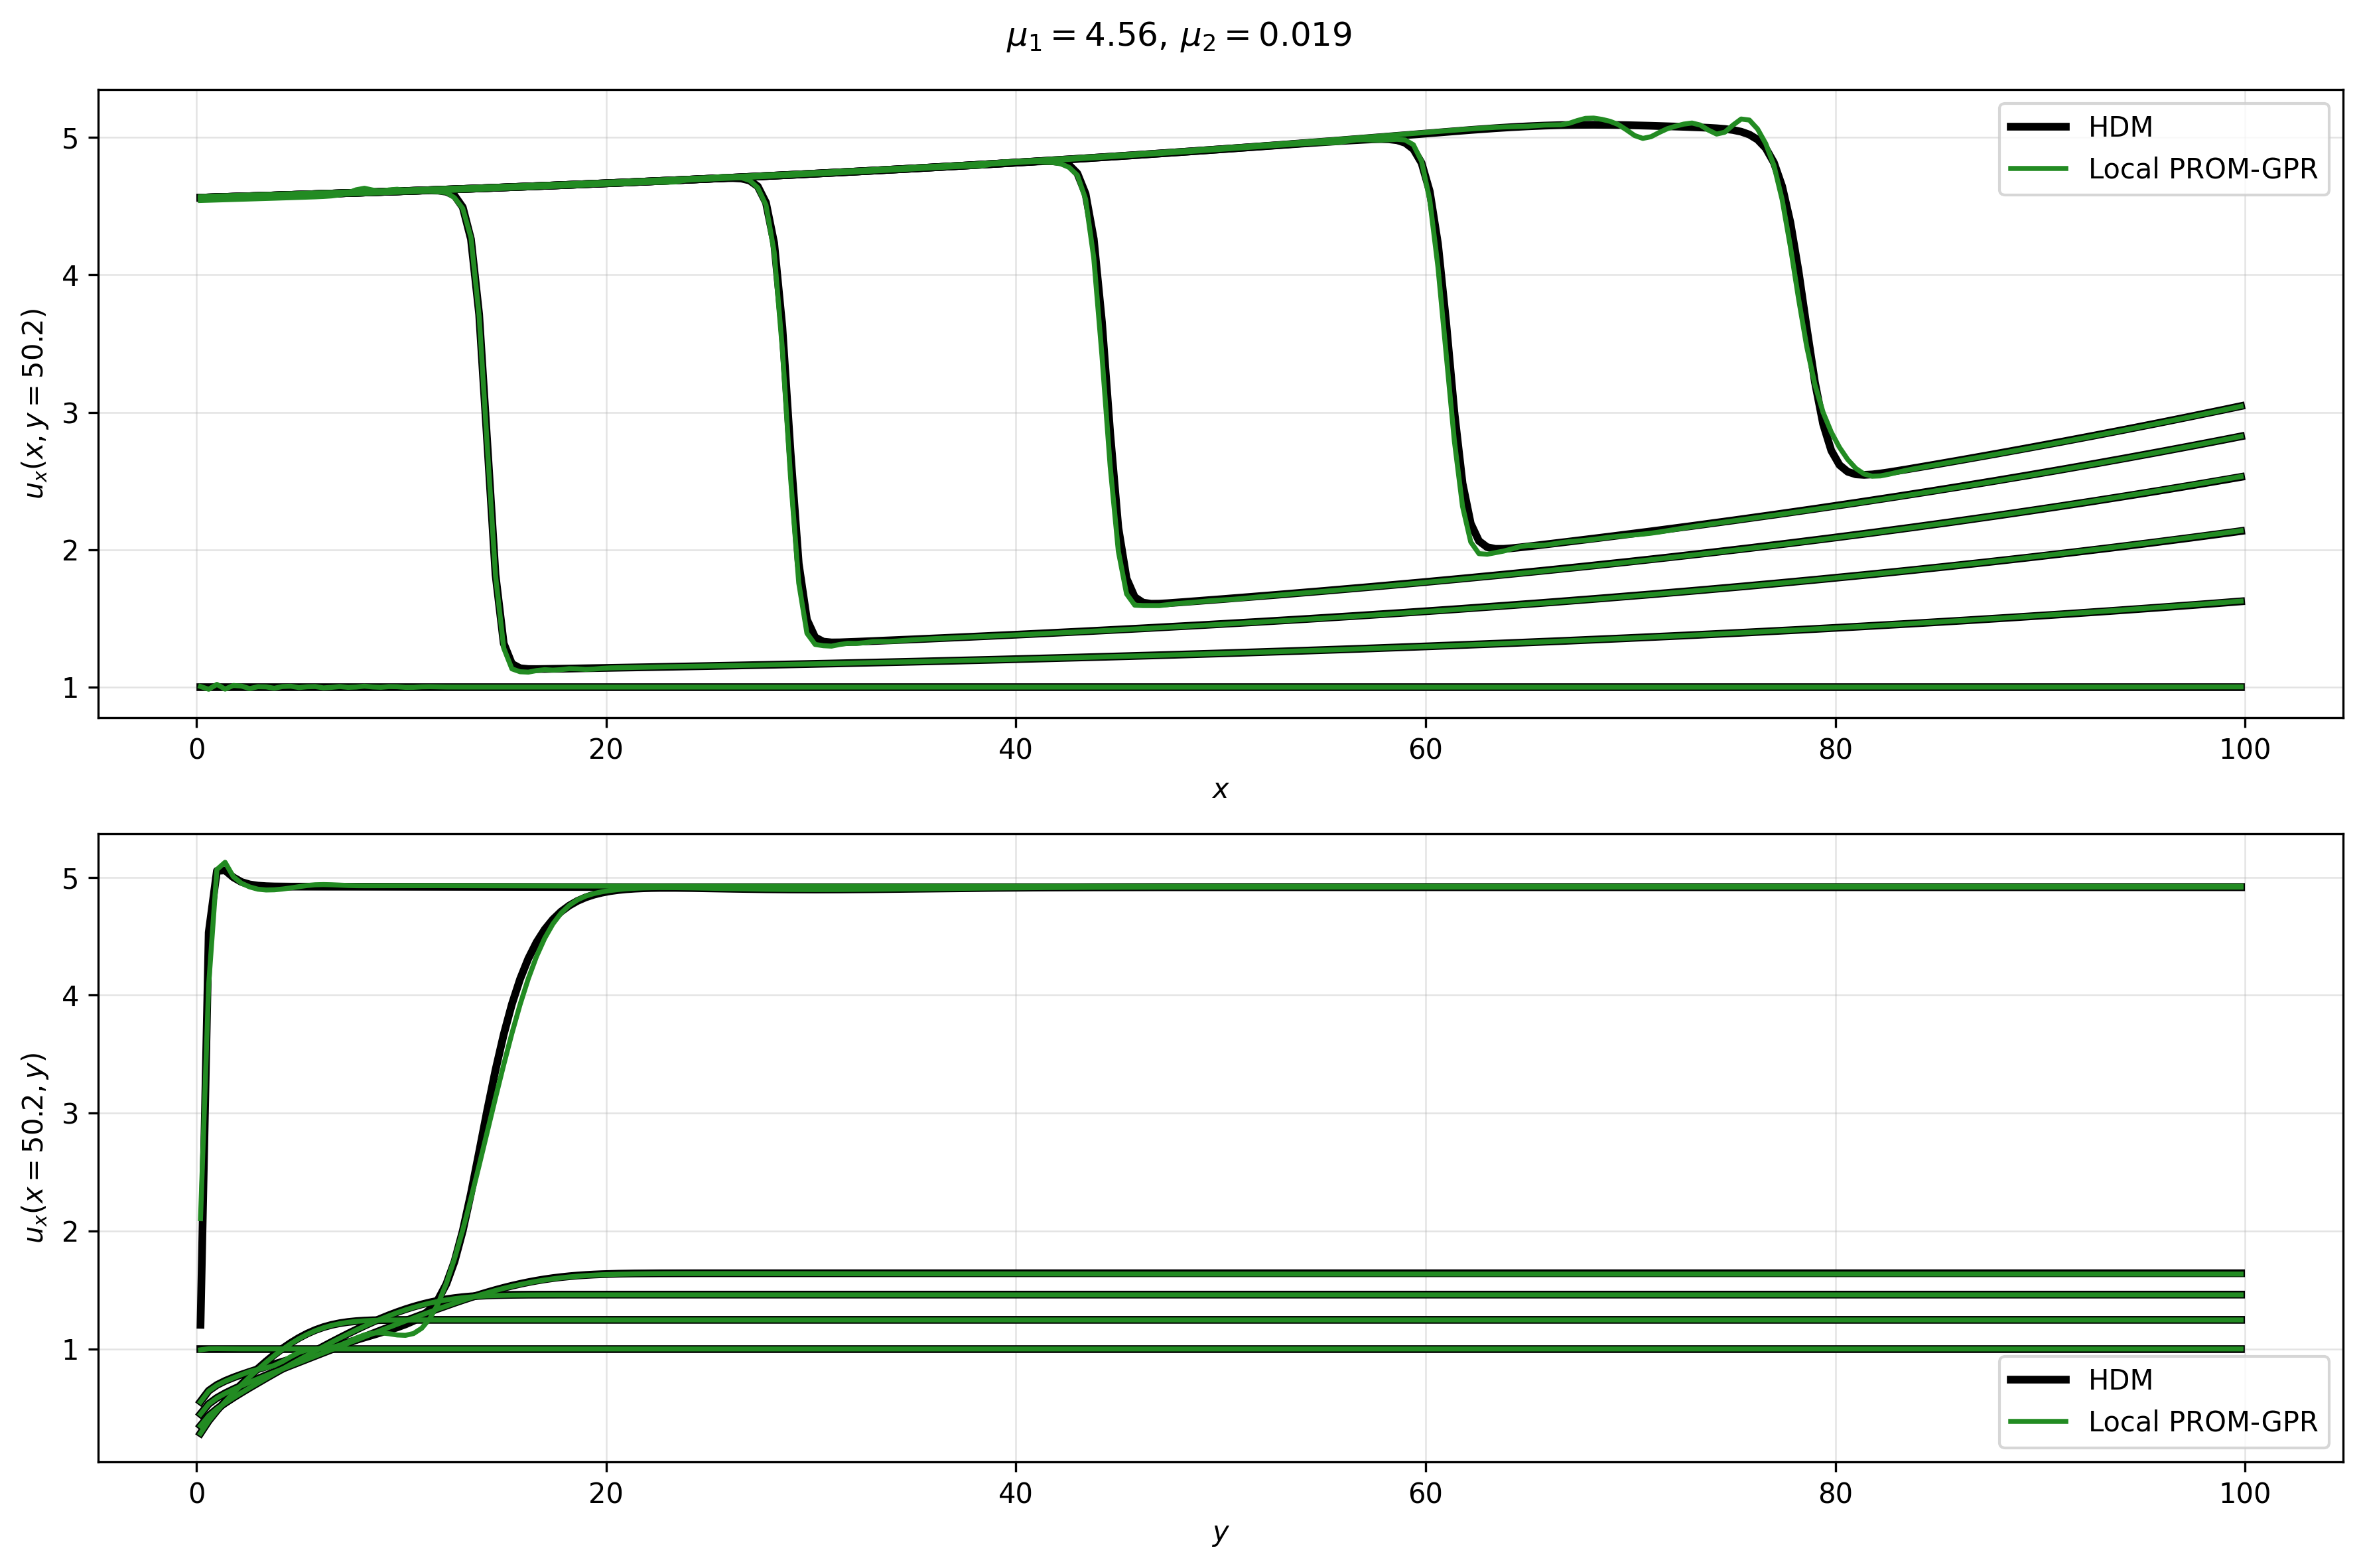
\includegraphics[width=0.80\textwidth]{Figures/local_prom_gpr_vs_hdm.png}
\vspace{0.2em}

{\scriptsize $\mathbb{RE}_{2,\mathbf{u}}=0.823\%$ \quad $t=102.035$ s $(1.701$ min$)$ \quad speedup $=7.357\times$}
\end{frame}

\begin{frame}{PROM-POD-DL Solution ($250\times250$): $\boldsymbol{\mu}=(4.56,\,0.019)$}
\centering
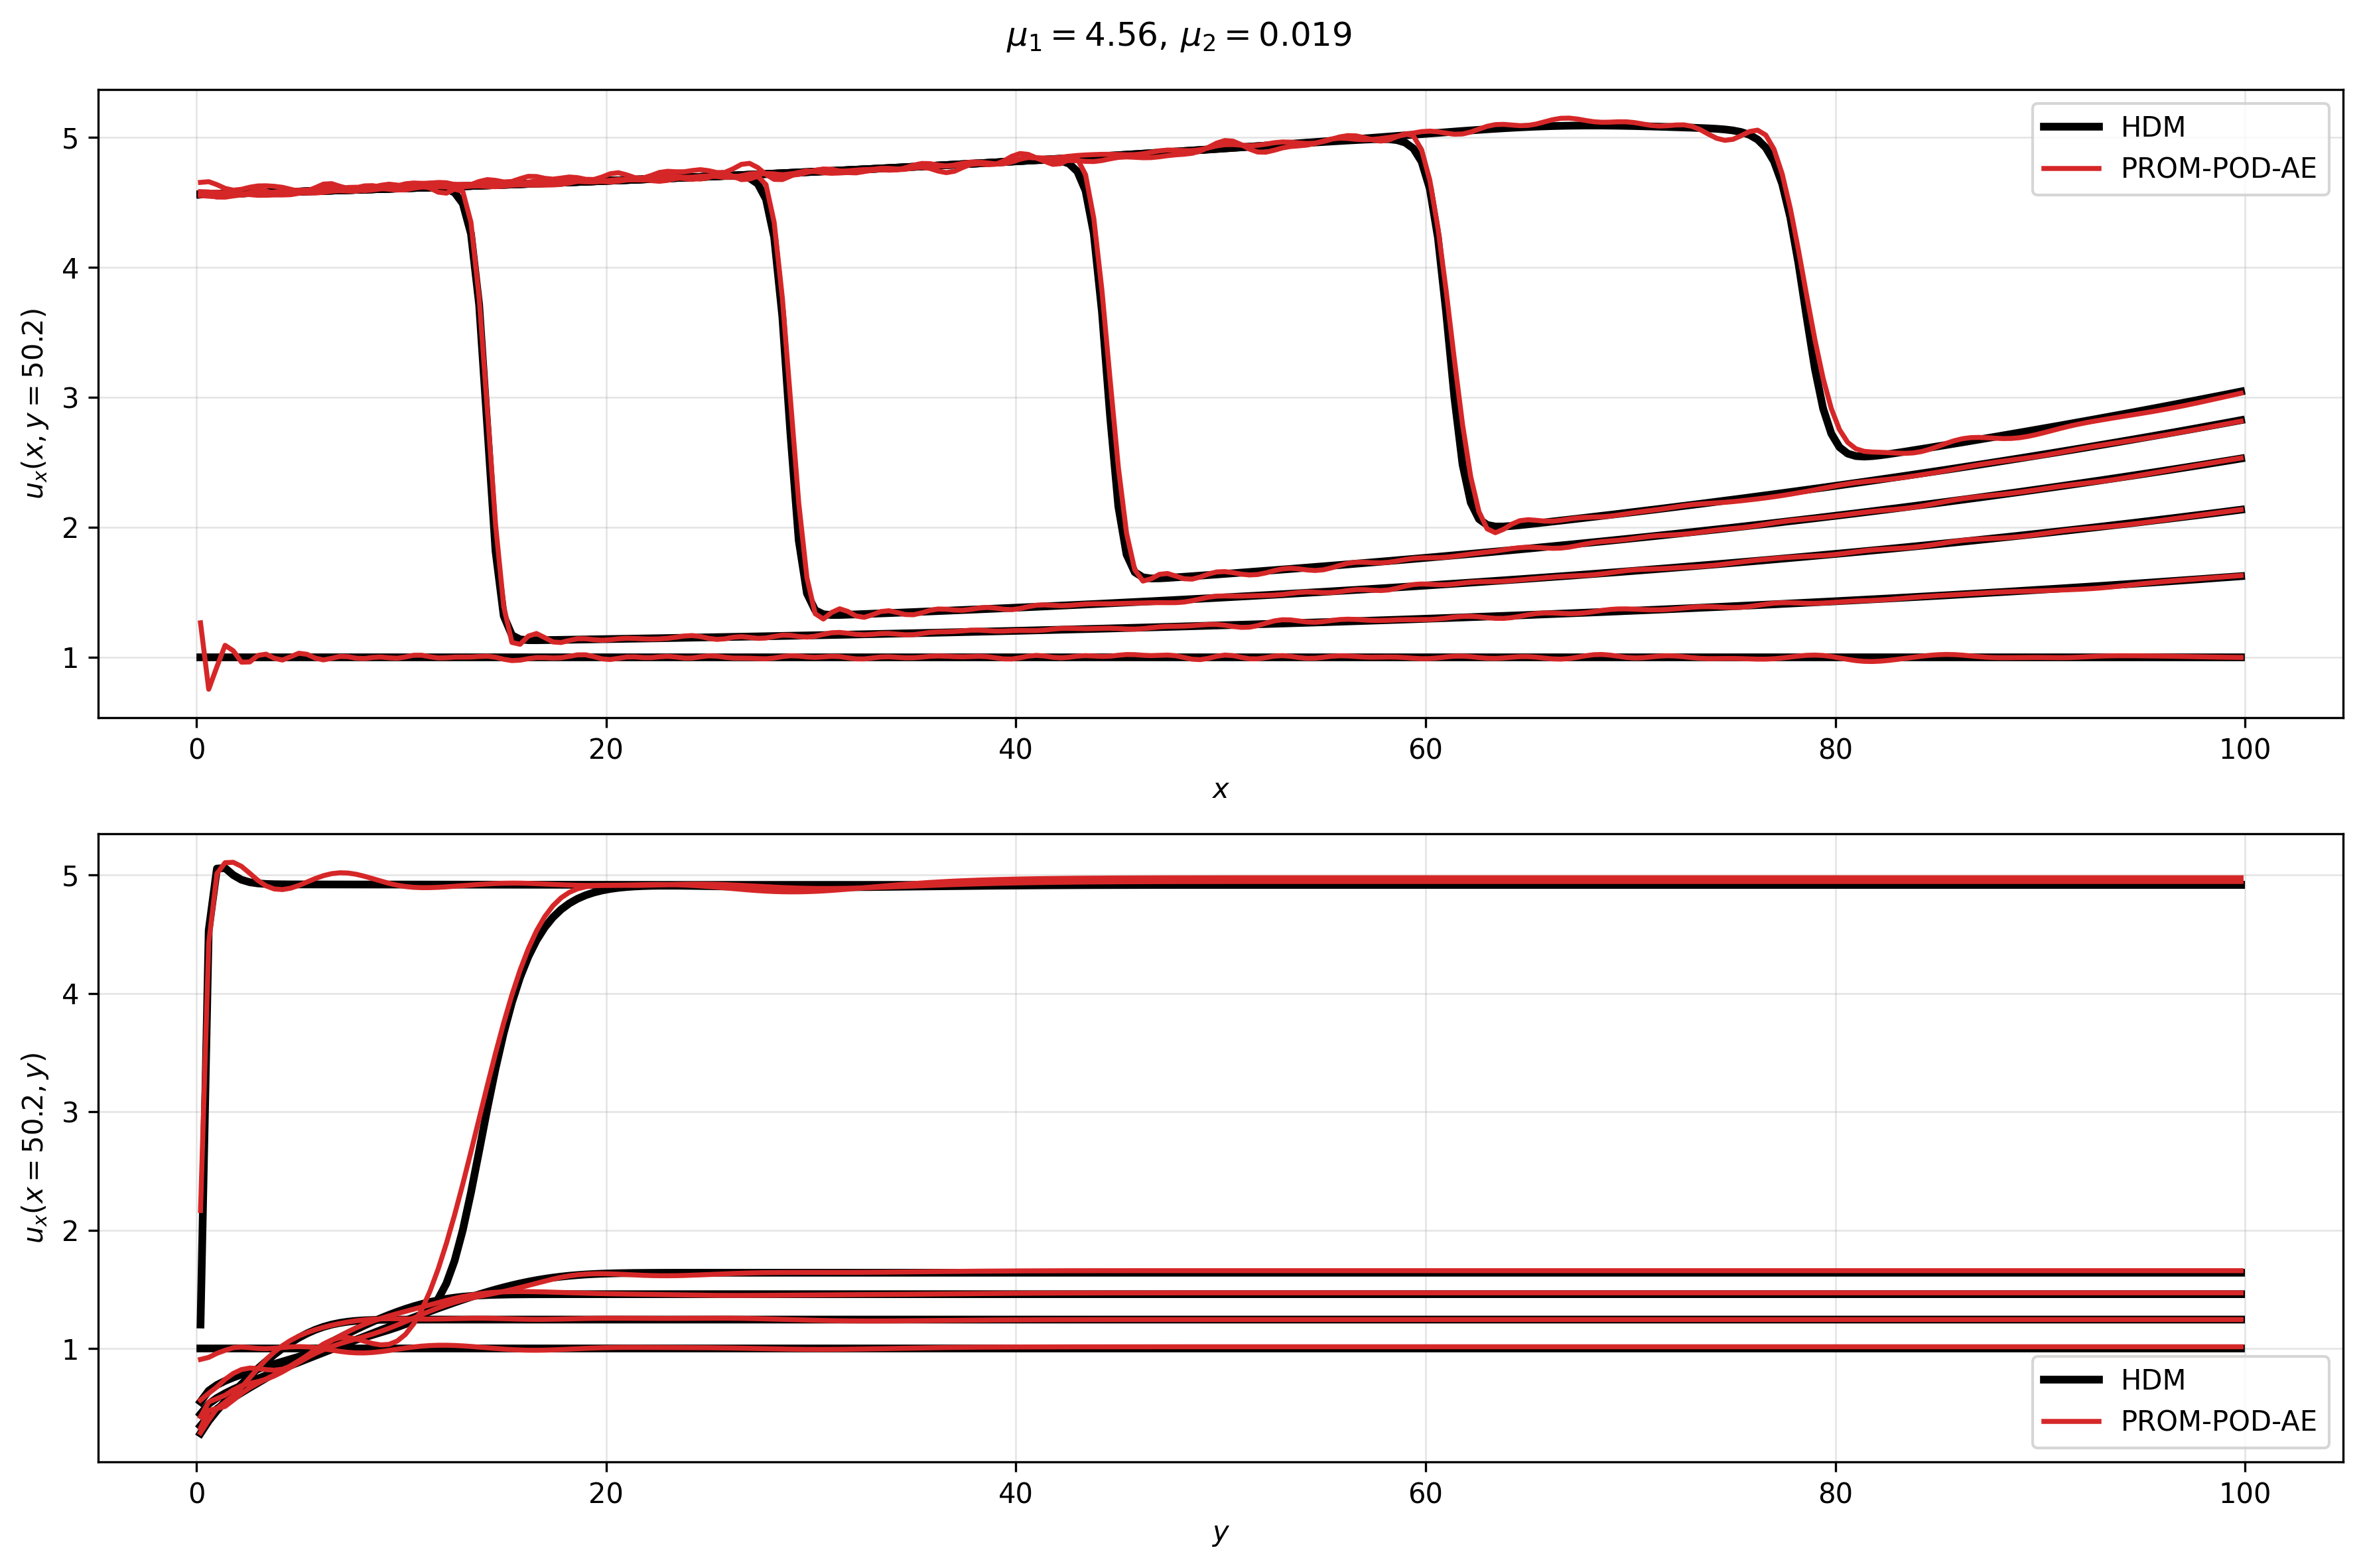
\includegraphics[width=0.80\textwidth]{Figures/prom_dl_vs_hdm.png}
\vspace{0.2em}

{\scriptsize $\mathbb{RE}_{2,\mathbf{u}}=1.242\%$ \quad $t=126.934$ s $(2.116$ min$)$ \quad speedup $=5.914\times$}
\end{frame}

\appendix

\begin{frame}{Appendix scope}
\small
Main online results use the affine cheap selector from the local linear PROM slides.
This appendix records exact extensions for local QPROM and local PROM-GPR.
They are included for completeness and are not used in the reported timings/errors.
\end{frame}

\begin{frame}{Local QPROM criterion}
\small
Assume current active cluster $k^-$ and reconstructed state
\[
\mathbf u^s
=
\mathbf u_{0,k^-}
+
\mathbf V_{k^-}\mathbf q_{k^-}
+
\mathbf H_{k^-}(\mathbf q_{k^-}\otimes \mathbf q_{k^-}).
\]

Choose the next cluster by nearest centroid $\mathbf u_{c,\ell}$, $\ell=1,\dots,N_c$:
\[
k^+
=
\arg\min_{\ell}
\|\mathbf u^s-\mathbf u_{c,\ell}\|_2^2.
\]

Define
\[
\mathbf a_\ell:=\mathbf u_{0,k^-}-\mathbf u_{c,\ell},
\quad
\mathbf b:=\mathbf V_{k^-}\mathbf q_{k^-},
\quad
\mathbf h:=\mathbf H_{k^-}(\mathbf q_{k^-}\otimes \mathbf q_{k^-}).
\]
Then
\[
k^+=\arg\min_\ell \|\mathbf a_\ell+\mathbf b+\mathbf h\|_2^2.
\]
\end{frame}

\begin{frame}{Local QPROM selector expansion}
\scriptsize
\[
\|\mathbf a_\ell+\mathbf b+\mathbf h\|_2^2
=
\|\mathbf a_\ell\|_2^2
+
2\,\mathbf a_\ell^T\mathbf b
+
2\,\mathbf a_\ell^T\mathbf h
+
\|\mathbf b\|_2^2
+
2\,\mathbf b^T\mathbf h
+
\|\mathbf h\|_2^2.
\]
Terms independent of $\ell$ can be dropped in the minimization, so
\[
k^+
=
\arg\min_\ell
\left[
\|\mathbf a_\ell\|_2^2
+
2\,\mathbf a_\ell^T\mathbf b
+
2\,\mathbf a_\ell^T\mathbf h
\right].
\]
Equivalent original form:
\[
k^+
=
\arg\min_\ell
\Big[
\|\mathbf u_{0,k^-}-\mathbf u_{c,\ell}\|_2^2
+
2(\mathbf u_{0,k^-}-\mathbf u_{c,\ell})^T\mathbf V_{k^-}\mathbf q_{k^-}
\]
\[
\qquad\qquad\qquad
+
2(\mathbf u_{0,k^-}-\mathbf u_{c,\ell})^T
\mathbf H_{k^-}(\mathbf q_{k^-}\otimes\mathbf q_{k^-})
\Big].
\]
\end{frame}

\begin{frame}{Local QPROM selector (offline/online form)}
\small
Precompute offline
\[
\mathbf g_{k^-,\ell}:=\mathbf V_{k^-}^T(\mathbf u_{0,k^-}-\mathbf u_{c,\ell}),
\qquad
d_{k^-,\ell}:=\|\mathbf u_{0,k^-}-\mathbf u_{c,\ell}\|_2^2,
\]
and define $\mathbf m_{k^-,\ell}\in\mathbb R^{n_{k^-}^2}$ by
\[
\mathbf m_{k^-,\ell}^T(\mathbf q\otimes\mathbf q)
:=
(\mathbf u_{0,k^-}-\mathbf u_{c,\ell})^T\mathbf H_{k^-}(\mathbf q\otimes\mathbf q).
\]
Then online:
\[
k^+
=
\arg\min_\ell
\left(
2\,\mathbf g_{k^-,\ell}^T\mathbf q_{k^-}
+
2\,\mathbf m_{k^-,\ell}^T(\mathbf q_{k^-}\otimes\mathbf q_{k^-})
+
d_{k^-,\ell}
\right).
\]
\end{frame}

\begin{frame}{Local QPROM switch after a cluster change}
\small
If $k^+=k^-$, no transfer is needed.

If $k^+\neq k^-$, the transferred state
\[
\mathbf u^s
=
\mathbf u_{0,k^-}
+
\mathbf V_{k^-}\mathbf q_{k^-}
+
\mathbf H_{k^-}(\mathbf q_{k^-}\otimes\mathbf q_{k^-})
\]
must be re-expressed in the new quadratic local manifold
\[
\mathbf u
\approx
\mathbf u_{0,k^+}
+
\mathbf V_{k^+}\mathbf q
+
\mathbf H_{k^+}(\mathbf q\otimes\mathbf q).
\]
Hence the transfer is
\[
\mathbf q_{k^+}
=
\arg\min_{\mathbf q}
\left\|
\mathbf u^s
-
\left(
\mathbf u_{0,k^+}
+
\mathbf V_{k^+}\mathbf q
+
\mathbf H_{k^+}(\mathbf q\otimes\mathbf q)
\right)
\right\|_2^2,
\]
typically solved with Gauss--Newton.
\end{frame}

\begin{frame}{Local PROM-GPR criterion}
\small
Assume current active cluster $k^-$ and reconstructed state
\[
\mathbf u^s
=
\mathbf u_{0,k^-}
+
\mathbf V_{k^-}\mathbf q_{k^-}
+
\bar{\mathbf V}_{k^-}\bar{\mathbf q}_{k^-},
\qquad
\bar{\mathbf q}_{k^-}
=
\mathcal N_{\mathrm{GPR},k^-}(\mathbf q_{k^-}).
\]
Nearest-centroid criterion:
\[
k^+
=
\arg\min_{\ell=1,\dots,N_c}
\|\mathbf u^s-\mathbf u_{c,\ell}\|_2^2.
\]
With $\mathbf a_\ell:=\mathbf u_{0,k^-}-\mathbf u_{c,\ell}$,
\[
k^+
=
\arg\min_\ell
\left\|
\mathbf a_\ell
+
\mathbf V_{k^-}\mathbf q_{k^-}
+
\bar{\mathbf V}_{k^-}\bar{\mathbf q}_{k^-}
\right\|_2^2.
\]
\end{frame}

\begin{frame}{Local PROM-GPR selector expansion}
\scriptsize
\[
\|\mathbf u^s-\mathbf u_{c,\ell}\|_2^2
=
\|\mathbf u_{0,k^-}-\mathbf u_{c,\ell}\|_2^2
+
2(\mathbf u_{0,k^-}-\mathbf u_{c,\ell})^T\mathbf V_{k^-}\mathbf q_{k^-}
\]
\[
+
2(\mathbf u_{0,k^-}-\mathbf u_{c,\ell})^T\bar{\mathbf V}_{k^-}\bar{\mathbf q}_{k^-}
+
\mathbf q_{k^-}^T\mathbf V_{k^-}^T\mathbf V_{k^-}\mathbf q_{k^-}
\]
\[
+
2\,\mathbf q_{k^-}^T\mathbf V_{k^-}^T\bar{\mathbf V}_{k^-}\bar{\mathbf q}_{k^-}
+
\bar{\mathbf q}_{k^-}^T\bar{\mathbf V}_{k^-}^T\bar{\mathbf V}_{k^-}\bar{\mathbf q}_{k^-}.
\]
Dropping terms independent of $\ell$:
\[
k^+
=
\arg\min_\ell
\Big[
\|\mathbf u_{0,k^-}-\mathbf u_{c,\ell}\|_2^2
+
2(\mathbf u_{0,k^-}-\mathbf u_{c,\ell})^T\mathbf V_{k^-}\mathbf q_{k^-}
\]
\[
\qquad\qquad
+
2(\mathbf u_{0,k^-}-\mathbf u_{c,\ell})^T\bar{\mathbf V}_{k^-}\bar{\mathbf q}_{k^-}
\Big].
\]
\end{frame}

\begin{frame}{Local PROM-GPR selector (offline/online form)}
\small
Precompute offline
\[
\mathbf g_{k^-,\ell}:=\mathbf V_{k^-}^T(\mathbf u_{0,k^-}-\mathbf u_{c,\ell}),
\qquad
\bar{\mathbf g}_{k^-,\ell}:=\bar{\mathbf V}_{k^-}^T(\mathbf u_{0,k^-}-\mathbf u_{c,\ell}),
\]
\[
d_{k^-,\ell}:=\|\mathbf u_{0,k^-}-\mathbf u_{c,\ell}\|_2^2.
\]
Then online:
\[
k^+
=
\arg\min_\ell
\left(
2\,\mathbf g_{k^-,\ell}^T\mathbf q_{k^-}
+
2\,\bar{\mathbf g}_{k^-,\ell}^T\bar{\mathbf q}_{k^-}
+
d_{k^-,\ell}
\right).
\]
with
\[
\bar{\mathbf q}_{k^-}=\mathcal N_{\mathrm{GPR},k^-}(\mathbf q_{k^-}).
\]
\end{frame}

\begin{frame}{Local PROM-GPR switch after a cluster change}
\small
If $k^+=k^-$, no transfer is needed.

If $k^+\neq k^-$, the transferred state
\[
\mathbf u^s
=
\mathbf u_{0,k^-}
+
\mathbf V_{k^-}\mathbf q_{k^-}
+
\bar{\mathbf V}_{k^-}\mathcal N_{\mathrm{GPR},k^-}(\mathbf q_{k^-})
\]
must be re-expressed in the new local manifold
\[
\mathbf u
\approx
\mathbf u_{0,k^+}
+
\mathbf V_{k^+}\mathbf q
+
\bar{\mathbf V}_{k^+}\mathcal N_{\mathrm{GPR},k^+}(\mathbf q).
\]
Hence the transfer is
\[
\mathbf q_{k^+}
=
\arg\min_{\mathbf q}
\left\|
\mathbf u^s
-
\left(
\mathbf u_{0,k^+}
+
\mathbf V_{k^+}\mathbf q
+
\bar{\mathbf V}_{k^+}\mathcal N_{\mathrm{GPR},k^+}(\mathbf q)
\right)
\right\|_2^2,
\]
typically solved with Gauss--Newton.
\end{frame}

\end{document}
